\documentclass[
  shortnames]{jss}

%% recommended packages
\usepackage{orcidlink,thumbpdf,lmodern}

\usepackage[utf8]{inputenc}

\author{
H. Sherry Zhang\\Monash University \And Dianne Cook\\Monash University \AND Ursula Laa\\University of Natural Resources and Life Sciences \AND Nicolas Langrené\\BNU-HKBU United International College \And Patricia Menéndez\\Monash University
}
\title{\pkg{cubble}: An \proglang{R} Package for Organizing and Wrangling Multivariate Spatio-temporal Data}

\Plainauthor{H. Sherry Zhang, Dianne Cook, Ursula Laa, Nicolas Langrené, Patricia Menéndez}
\Plaintitle{cubble: An R Package for Organizing and Wrangling Multivariate Spatio-temporal Data}


\Abstract{
Multivariate spatio-temporal data refers to multiple measurements taken across space and time. For many analyses, spatial and time components can be separately studied: for example, to explore the temporal trend of one variable for a single spatial location, or to model the spatial distribution of one variable at a given time. However for some studies, it is important to analyze different aspects of the spatio-temporal data simultaneously, like for instance, temporal trends of multiple variables across locations. In order to facilitate the study of different portions or combinations of spatio-temporal data, we introduce a new class, \code{cubble}, with a suite of functions enabling easy slicing and dicing on different spatio-temporal components. The proposed \code{cubble} class ensures that all the components of the data are easy to access and manipulate while providing flexibility for data analysis. In addition, the \pkg{cubble} package facilitates visual and numerical explorations of the data while easing data wrangling and modelling. The \code{cubble} class and the functions provided in the \pkg{cubble} \proglang{R} package equip users with the capability to handle hierarchical spatial and temporal structures. The \code{cubble} class and the tools implemented in the package are illustrated with different examples of Australian climate data.
}

\Keywords{spatial, temporal, spatio temporal, \proglang{R}, environmental data, exploratory data analysis}
\Plainkeywords{spatial, temporal, spatio temporal, R, environmental data, exploratory data analysis}

%% publication information
%% \Volume{50}
%% \Issue{9}
%% \Month{June}
%% \Year{2012}
%% \Submitdate{}
%% \Acceptdate{2012-06-04}

\Address{
    H. Sherry Zhang\\
    Monash University\\
    21 Chancellors Walk, Clayton VIC 3800 Australia\\
  E-mail: \email{huize.zhang@monash.edu}\\
  
      Dianne Cook\\
    Monash University\\
    21 Chancellors Walk, Clayton VIC 3800 Australia\\
  E-mail: \href{mailto:dicook@monash.edu}{\nolinkurl{dicook@monash.edu}}\\
  
      Ursula Laa\\
    University of Natural Resources and Life Sciences\\
    Gregor-Mendel-Straße 33, 1180 Wien, Austria\\
  E-mail: \href{mailto:ursula.laa@boku.ac.at}{\nolinkurl{ursula.laa@boku.ac.at}}\\
  
      Nicolas Langrené\\
    BNU-HKBU United International College\\
    2000 Jintong Road, Tangjiawan, Zhuhai, Guangdong Province, China\\
  E-mail: \href{mailto:nicolaslangrene@uic.edu.cn}{\nolinkurl{nicolaslangrene@uic.edu.cn}}\\
  
      Patricia Menéndez\\
    Monash University\\
    21 Chancellors Walk, Clayton VIC 3800 Australia\\
  E-mail: \href{mailto:patricia.menendez@monash.edu}{\nolinkurl{patricia.menendez@monash.edu}}\\
  
  }

% Pandoc syntax highlighting
\usepackage{color}
\usepackage{fancyvrb}
\newcommand{\VerbBar}{|}
\newcommand{\VERB}{\Verb[commandchars=\\\{\}]}
\DefineVerbatimEnvironment{Highlighting}{Verbatim}{commandchars=\\\{\}}
% Add ',fontsize=\small' for more characters per line
\usepackage{framed}
\definecolor{shadecolor}{RGB}{248,248,248}
\newenvironment{Shaded}{\begin{snugshade}}{\end{snugshade}}
\newcommand{\AlertTok}[1]{\textcolor[rgb]{0.94,0.16,0.16}{#1}}
\newcommand{\AnnotationTok}[1]{\textcolor[rgb]{0.56,0.35,0.01}{\textbf{\textit{#1}}}}
\newcommand{\AttributeTok}[1]{\textcolor[rgb]{0.77,0.63,0.00}{#1}}
\newcommand{\BaseNTok}[1]{\textcolor[rgb]{0.00,0.00,0.81}{#1}}
\newcommand{\BuiltInTok}[1]{#1}
\newcommand{\CharTok}[1]{\textcolor[rgb]{0.31,0.60,0.02}{#1}}
\newcommand{\CommentTok}[1]{\textcolor[rgb]{0.56,0.35,0.01}{\textit{#1}}}
\newcommand{\CommentVarTok}[1]{\textcolor[rgb]{0.56,0.35,0.01}{\textbf{\textit{#1}}}}
\newcommand{\ConstantTok}[1]{\textcolor[rgb]{0.00,0.00,0.00}{#1}}
\newcommand{\ControlFlowTok}[1]{\textcolor[rgb]{0.13,0.29,0.53}{\textbf{#1}}}
\newcommand{\DataTypeTok}[1]{\textcolor[rgb]{0.13,0.29,0.53}{#1}}
\newcommand{\DecValTok}[1]{\textcolor[rgb]{0.00,0.00,0.81}{#1}}
\newcommand{\DocumentationTok}[1]{\textcolor[rgb]{0.56,0.35,0.01}{\textbf{\textit{#1}}}}
\newcommand{\ErrorTok}[1]{\textcolor[rgb]{0.64,0.00,0.00}{\textbf{#1}}}
\newcommand{\ExtensionTok}[1]{#1}
\newcommand{\FloatTok}[1]{\textcolor[rgb]{0.00,0.00,0.81}{#1}}
\newcommand{\FunctionTok}[1]{\textcolor[rgb]{0.00,0.00,0.00}{#1}}
\newcommand{\ImportTok}[1]{#1}
\newcommand{\InformationTok}[1]{\textcolor[rgb]{0.56,0.35,0.01}{\textbf{\textit{#1}}}}
\newcommand{\KeywordTok}[1]{\textcolor[rgb]{0.13,0.29,0.53}{\textbf{#1}}}
\newcommand{\NormalTok}[1]{#1}
\newcommand{\OperatorTok}[1]{\textcolor[rgb]{0.81,0.36,0.00}{\textbf{#1}}}
\newcommand{\OtherTok}[1]{\textcolor[rgb]{0.56,0.35,0.01}{#1}}
\newcommand{\PreprocessorTok}[1]{\textcolor[rgb]{0.56,0.35,0.01}{\textit{#1}}}
\newcommand{\RegionMarkerTok}[1]{#1}
\newcommand{\SpecialCharTok}[1]{\textcolor[rgb]{0.00,0.00,0.00}{#1}}
\newcommand{\SpecialStringTok}[1]{\textcolor[rgb]{0.31,0.60,0.02}{#1}}
\newcommand{\StringTok}[1]{\textcolor[rgb]{0.31,0.60,0.02}{#1}}
\newcommand{\VariableTok}[1]{\textcolor[rgb]{0.00,0.00,0.00}{#1}}
\newcommand{\VerbatimStringTok}[1]{\textcolor[rgb]{0.31,0.60,0.02}{#1}}
\newcommand{\WarningTok}[1]{\textcolor[rgb]{0.56,0.35,0.01}{\textbf{\textit{#1}}}}

% tightlist command for lists without linebreak
\providecommand{\tightlist}{%
  \setlength{\itemsep}{0pt}\setlength{\parskip}{0pt}}

% From pandoc table feature
\usepackage{longtable,booktabs,array}
\usepackage{calc} % for calculating minipage widths
% Correct order of tables after \paragraph or \subparagraph
\usepackage{etoolbox}
\makeatletter
\patchcmd\longtable{\par}{\if@noskipsec\mbox{}\fi\par}{}{}
\makeatother
% Allow footnotes in longtable head/foot
\IfFileExists{footnotehyper.sty}{\usepackage{footnotehyper}}{\usepackage{footnote}}
\makesavenoteenv{longtable}



\usepackage{amsmath} \usepackage{array} \usepackage{xcolor} \newcommand{\sherry}[1]{\textcolor{magenta}{#1}}

\begin{document}



\newpage

\hypertarget{introduction}{%
\section{Introduction}\label{introduction}}

Spatio-temporal data has a spatial component referring to the location of each observation and a temporal component that is recorded at regular or irregular time intervals. It may also include multiple variables measured at each spatial and temporal values. With spatio-temporal data, one can fix the time to explore the spatial features of the data, fix the spatial location/s to explore temporal aspects, or dynamically explore the space and time simultaneously.

In order to computationally explore the spatial, temporal and spatio-temporal faces of such data, the data needs to be stored and represented under a specific data object that allows the user to query, group and dissect all the data faces.

The Comprehensive \proglang{R} Archive Network (CRAN) task view SpatioTemporal \citep{ctvspatiotemporal} gathers information about \proglang{R} packages designed for spatio-temporal data and it has a section on \emph{Representing data} that lists existing spatio-temporal data representations used in \proglang{R}. Among them, \citet{spacetime} summarises spatio-temporal data into three forms: time-wide, space-wide, and long formats. The associated package \pkg{spacetime} \citep{spacetime} implements four spatio-temporal layouts (full grid, sparse grid, irregular, and trajectory) to handle different space and time combinations. The package \pkg{stars} \citep{stars} has a new implementation to use dense arrays to represent spatio-temporal cubes. It also interfaces with the package \pkg{sf} \citep{sf}, commonly used for wrangling spatial data, and the \pkg{tidyverse} \citep{tidyverse} suite for general data wrangling and visualization in \proglang{R}.

Still, the data representation for spatio-temporal data can be further extended and there are two reasons for this. Firstly, the raw data sourced in the wild is less often presented in any one of the layouts above, and fitting the raw data into a data object can sometimes be difficult. More often, spatio-temporal data are collected in separate 2D tables and analysts need to assemble them into a whole piece before exploring the data. Examples of components of spatio-temporal data can be 1) areal data recording the shape of a collection of areas of interest; 2) geostatistical data storing the longitude and latitude coordinates of locations, typically also with other metadata related to the location, and; 3) temporal data of each location across time.

The other reason is about tidy data concepts \citep{tidydata} and how they should be applied to spatio-temporal data. According to the tidy data principles, data should be structured into 1) one row per observation, 2) one column per variable, and 3) one type of data per table. The long form data is preferred over wide data form given the downstream packages such as \pkg{dplyr} \citep{dplyr} and \pkg{ggplot2} \citep{ggplot2} for data wrangling and visualization. However, the long form can be inefficient to store feature geometries, especially for large multipolygons for hourly, daily or sub-daily periods over years, which are extensively collected and handled, for example in time series analysis. This poses the question of how to arrange spatial and temporal variables in a way that would make data wrangling, visualizing and analyzing spatio-temporal data easier.

This paper presents a new \proglang{R} package, \pkg{cubble}, which addresses the two issues mentioned above. In the package, a new class, also called cubble, is proposed to organize spatial and temporal variables as two forms of a single data object so that they can be wrangled separately or combined while being kept synchronized. Among the four spacetime layouts in \citet{spacetime}, the \code{cubble} class can be applied to full grid, sparse grid, or irregular, but not trajectory, which is outside the scope of this work. The software is available from the Comprehensive \proglang{R} Archive Network (CRAN) at \url{https://CRAN.R-project.org/package=cubble}.

The rest of the paper is organized as follows: Section \ref{cubble} presents the main design and functionality of the \pkg{cubble} package. Section \ref{others} explains how the \pkg{cubble} package deals with more advanced considerations, including data with hierarchical structure, data matching and how the package fits with existing static and interactive visualization tools. Moreover we also illustrate how the \pkg{cubble} package deals with spatio-temporal data transformations. Section \ref{examples} uses Australian weather station data and river level data as examples to demonstrate the use of the package. An example of how the \pkg{cubble} package handles Network Common Data Form (NetCDF) data is also provided. Section \ref{conclude} discuss the paper contributions and future directions.

\hypertarget{cubble}{%
\section{The cubble package}\label{cubble}}

\hypertarget{object}{%
\subsection{The cubble object}\label{object}}

\emph{the conceptual framework + nested and long form as per the design vignette}

\begin{itemize}
\tightlist
\item
  diagram,
\item
  two forms: long/ nested - spatial/ temporal
\item
  attributes
\item
  headers
\end{itemize}

The \code{cubble} class is an S3 class \citep{advr} built on the \code{tibble} class, specifically to organize spatio-temporal data. The \code{cubble} class uses an attribute ``form'', to arrange the spatial or temporal data components tidily. The form attribute can take a value of either ``nested'' or ``long''. The nested \code{cubble} is a subclass of rowwise \code{tibble} (\code{rowwise_df}). It arranges each spatial site in a row, and uses list columns to store the feature geometry and the temporal information. The long \code{cubble} is a subclass of grouped \code{tibble} (\code{grouped_df}), which expands the temporal information into the long form and stores the spatial information in a ``spatial'' attribute.

The arguments \code{key} and \code{index} follow the conventions in the \pkg{tsibble} package to describe the temporal order and multiple series while \code{coords} specifies the spatial location of each site.

\begin{CodeChunk}
\begin{CodeInput}
R> cb_nested
\end{CodeInput}
\begin{CodeOutput}
# cubble:   key: id [3], index: date, nested form
# extent:   [144.8321, -37.98, 145.0964, -37.6655]
# temporal: prcp [dbl], tmax [dbl], tmin [dbl]
  id           long   lat  elev name              wmo_id ts      
  <chr>       <dbl> <dbl> <dbl> <chr>              <dbl> <list>  
1 ASN00086038  145. -37.7  78.4 essendon airport   95866 <tibble>
2 ASN00086077  145. -38.0  12.1 moorabbin airport  94870 <tibble>
3 ASN00086282  145. -37.7 113.  melbourne airport  94866 <tibble>
\end{CodeOutput}
\begin{CodeInput}
R> class(cb_nested)
\end{CodeInput}
\begin{CodeOutput}
[1] "spatial_cubble_df" "cubble_df"         "rowwise_df"       
[4] "tbl_df"            "tbl"               "data.frame"       
\end{CodeOutput}
\end{CodeChunk}

Printing a \code{cubble} object provides some information about the data. Here \code{id} is the variable name to identify each location and there are five unique locations. The bounding box is \code{[115.97, -32.94, 133.55, -12.42]} and provides information about the coordinates in the data. The third row shows the name and type of all variables nested in the \code{ts} column. In this example, it includes \code{date [date], prcp [dbl], tmax [dbl], tmin [dbl]}.

\begin{CodeChunk}
\begin{CodeInput}
R> cb_long
\end{CodeInput}
\begin{CodeOutput}
# cubble:  key: id [3], index: date, long form
# extent:  2020-01-01 -- 2020-01-10 [1D], no gaps
# spatial: long [dbl], lat [dbl], elev [dbl], name [chr], wmo_id
#   [dbl]
  id          date        prcp  tmax  tmin
  <chr>       <date>     <dbl> <dbl> <dbl>
1 ASN00086038 2020-01-01     0  26.8  11  
2 ASN00086038 2020-01-02     0  26.3  12.2
3 ASN00086038 2020-01-03     0  34.5  12.7
4 ASN00086038 2020-01-04     0  29.3  18.8
5 ASN00086038 2020-01-05    18  16.1  12.5
# i 25 more rows
\end{CodeOutput}
\begin{CodeInput}
R> class(cb_long)
\end{CodeInput}
\begin{CodeOutput}
[1] "temporal_cubble_df" "cubble_df"          "tbl_df"            
[4] "tbl"                "data.frame"        
\end{CodeOutput}
\end{CodeChunk}

\hypertarget{create}{%
\subsection{Creation and coercion}\label{create}}

\hypertarget{creating-from-separate-spatial-and-temporal-tables}{%
\subsubsection{Creating from separate spatial and temporal tables}\label{creating-from-separate-spatial-and-temporal-tables}}

Spatio-temporal data may arrive in separate tables for analysts. For example, in climate data, analysts may initially receive station data containing geographic location information, variables recorded and their recording periods. They can then query the temporal variables using the stations of interest to obtain the corresponding temporal data. Alternatively, analyses may begin as purely spatial or temporal, and analysts may obtain additional temporal or spatial data to expand the result to spatio-temporal.

The function \code{make_cubble()} composes a \code{cubble} object from a spatial table (\code{spatial}) and a temporal table (\code{temporal}) with the three attributes introduced in the subsection \ref{object}: \code{key}, \code{index}, and \code{coords}. The following code creates the nested \code{cubble} object shown previously:

\begin{CodeChunk}
\begin{CodeInput}
R> make_cubble(spatial = stations, temporal = meteo,
+             key = id, index = date, coords = c(long, lat))
\end{CodeInput}
\end{CodeChunk}

The \code{key} and \code{index} arguments corresponds to the \code{tsibble} counterpart and \code{coords} derives from the geometry column in an \code{sf} object. Hence, the corresponding argument can be safely omitted, if the spatial data is an \code{sf} object, i.e.~\code{stations_sf}, or the temporal data is a \code{tsibble} object, i.e.~\code{meteo_ts}. The \code{sf} and \code{tsibble} class from the input will be carried over to the \code{cubble} object:

\begin{CodeChunk}
\begin{CodeInput}
R> (res <- make_cubble(spatial = stations_sf, temporal = meteo_ts))
\end{CodeInput}
\begin{CodeOutput}
# cubble:   key: id [3], index: date, nested form, [sf]
# extent:   [144.8321, -37.98, 145.0964, -37.6655]
# temporal: prcp [dbl], tmax [dbl], tmin [dbl]
  id           long   lat  elev name  wmo_id            geometry
  <chr>       <dbl> <dbl> <dbl> <chr>  <dbl>         <POINT [°]>
1 ASN00086038  145. -37.7  78.4 esse~  95866 (144.9066 -37.7276)
2 ASN00086077  145. -38.0  12.1 moor~  94870   (145.0964 -37.98)
3 ASN00086282  145. -37.7 113.  melb~  94866 (144.8321 -37.6655)
# i 1 more variable: ts <list>
\end{CodeOutput}
\begin{CodeInput}
R> class(res)
\end{CodeInput}
\begin{CodeOutput}
[1] "spatial_cubble_df" "cubble_df"         "sf"               
[4] "tbl_df"            "tbl"               "data.frame"       
\end{CodeOutput}
\begin{CodeInput}
R> class(res$ts[[1]])
\end{CodeInput}
\begin{CodeOutput}
[1] "tbl_ts"     "tbl_df"     "tbl"        "data.frame"
\end{CodeOutput}
\end{CodeChunk}

\hypertarget{coercing-from-foregin-objects}{%
\subsubsection{Coercing from foregin objects}\label{coercing-from-foregin-objects}}

Spatio-temporal data in other foreign objects can be coerced into a \code{cubble} object with the function \code{as_cubble()}. This includes casting from a \code{tibble} or \code{data.frame} with both spatial and temporal information, a NetCDF object, a \code{stars} object \citep{stars}, and a \code{sftime} object \citep{sftime}. The two examples below show the casting from a tibble and a NetCDF object to a cubble object.

The dataset \code{climate_flat} joins the spatial data, \code{stations}, with the temporal data, \code{meteo}, into a single tibble object and it can be coerced into a cubble using:

\begin{CodeChunk}
\begin{CodeInput}
R> climate_flat |> as_cubble(key = id, index = date, coords = c(long, lat))
\end{CodeInput}
\end{CodeChunk}

The NetCDF data is another format commonly used for storing spatio-temporal data. In \proglang{R}, packages for wrangling NetCDF data include a high-level R interface: \pkg{ncdf4} \citep{ncdf4}, a low-level interface that calls a C-interface: \pkg{RNetCDF} \citep{rnetcdf}, and a tidyverse implementation: \pkg{tidync} \citep{tidync}. The code below casts a NetCDF object in the \code{ncdf4} class into a cubble object:

\begin{CodeChunk}
\begin{CodeInput}
R> path <- system.file("ncdf/era5-pressure.nc", package = "cubble")
R> raw <- ncdf4::nc_open(path)
R> as_cubble(raw)
\end{CodeInput}
\begin{CodeOutput}
# cubble:   key: id [26565], index: time, nested form
# extent:   [113, -53, 153, -12]
# temporal: q [dbl], z [dbl]
     id  long   lat ts              
  <int> <dbl> <dbl> <list>          
1     1  113    -12 <tibble [6 x 3]>
2     2  113.   -12 <tibble [6 x 3]>
3     3  114.   -12 <tibble [6 x 3]>
4     4  114.   -12 <tibble [6 x 3]>
5     5  114    -12 <tibble [6 x 3]>
# i 26,560 more rows
\end{CodeOutput}
\end{CodeChunk}

Sometimes, one may want to read in a subset of the NetCDF data and the argument \code{vars}, \code{long_range} and \code{lat_range} can be used to subset on the variable and the grid resolution:

\begin{CodeChunk}
\begin{CodeInput}
R> as_cubble(raw, vars = "q",
+           long_range = seq(-180, 180, 1), lat_range = seq(-90, 90, 1))
\end{CodeInput}
\end{CodeChunk}

We would recommend reducing to about 300 \(\times\) 300 grid points for three daily variables in one year. A 300 by 300 spatial grid can be a bounding box of {[}100, -80, 180, 0{]} at 0.25 degree resolution or a global bounding box {[}-180, -90, 180, -90{]} at 1 degree resolution.

\hypertarget{functions-and-methods-in-cubble}{%
\subsection{Functions and methods in cubble}\label{functions-and-methods-in-cubble}}

\emph{Print all the methods with methods(class = ``cubble\_df'')}

\hypertarget{dplyr-methods}{%
\subsubsection{dplyr methods}\label{dplyr-methods}}

The \pkg{dplyr} package has many tools for wrangling tidy data, many of which are useful in the spatio-temporal analysis. The \pkg{cubble} package provides methods that support the use of the following operations in the \pkg{dplyr} package on both the nested and long forms: \texttt{mutate}, \texttt{filter}, \texttt{summarise}, \texttt{select}, \texttt{arrange}, \texttt{rename}, \texttt{left\_join}, and the slice family (\texttt{slice\_*}).

The created \code{cubble} is a subclass of the \code{rowwise_df} class where each row forms a group. All the temporal variables are nested in a list column, hence it is also called the nested \code{cubble}. The rowwise structure makes it simpler to operate on the list using the \code{mutate()} syntax, which is simpler than the \code{purr::map()} when working with a list column. For example, calculating the number of rainy days can be done by:

\begin{CodeChunk}
\begin{CodeInput}
R> cb_nested |> mutate(rain_day = sum(ts$prcp != 0))
\end{CodeInput}
\begin{CodeOutput}
# cubble:   key: id [3], index: date, nested form
# extent:   [144.8321, -37.98, 145.0964, -37.6655]
# temporal: prcp [dbl], tmax [dbl], tmin [dbl]
  id           long   lat  elev name          wmo_id rain_day ts      
  <chr>       <dbl> <dbl> <dbl> <chr>          <dbl>    <int> <list>  
1 ASN00086038  145. -37.7  78.4 essendon air~  95866        3 <tibble>
2 ASN00086077  145. -38.0  12.1 moorabbin ai~  94870        3 <tibble>
3 ASN00086282  145. -37.7 113.  melbourne ai~  94866        3 <tibble>
\end{CodeOutput}
\end{CodeChunk}

\hypertarget{cubble-specific-methods}{%
\subsubsection{cubble specific methods}\label{cubble-specific-methods}}

The three cubble specific functions are \code{face_temporal()}, \code{face_spatial()}, and \code{unfold}.

The nested form can be used for those operations where the output is only indexed by the spatial identifier (\code{key}), but becomes inadequate when outputs need both a spatial and a temporal identifier (\code{key} and \code{index}). The \code{cubble} class also provides a long form, which expands the \code{ts} column and stores the spatial variables as an attribute. The function \code{face_temporal()} is used to switch from the nested \code{cubble} into the long one. The first row in Figure \ref{fig:face} illustrates this operation where the focus of the cube now changes from the site-variable face to the time-variable face. This code switches the \code{cubble} object just created into its long form:

\begin{CodeChunk}
\begin{CodeInput}
R> (cb_long <- cb_nested |> face_temporal())
\end{CodeInput}
\begin{CodeOutput}
# cubble:  key: id [3], index: date, long form
# extent:  2020-01-01 -- 2020-01-10 [1D], no gaps
# spatial: long [dbl], lat [dbl], elev [dbl], name [chr], wmo_id
#   [dbl]
  id          date        prcp  tmax  tmin
  <chr>       <date>     <dbl> <dbl> <dbl>
1 ASN00086038 2020-01-01     0  26.8  11  
2 ASN00086038 2020-01-02     0  26.3  12.2
3 ASN00086038 2020-01-03     0  34.5  12.7
4 ASN00086038 2020-01-04     0  29.3  18.8
5 ASN00086038 2020-01-05    18  16.1  12.5
# i 25 more rows
\end{CodeOutput}
\end{CodeChunk}

The first line in the header now shows it in the long form and the third line has been changed to display the name and type of spatial variables: \code{lat [dbl], long [dbl], elev [dbl], name [chr], wmo_id [dbl]}. Unlike the nested form, the long \code{cubble} is built from a \code{grouped_df} class where all the observations from the same site form a group.

\begin{CodeChunk}
\begin{figure}

{\centering 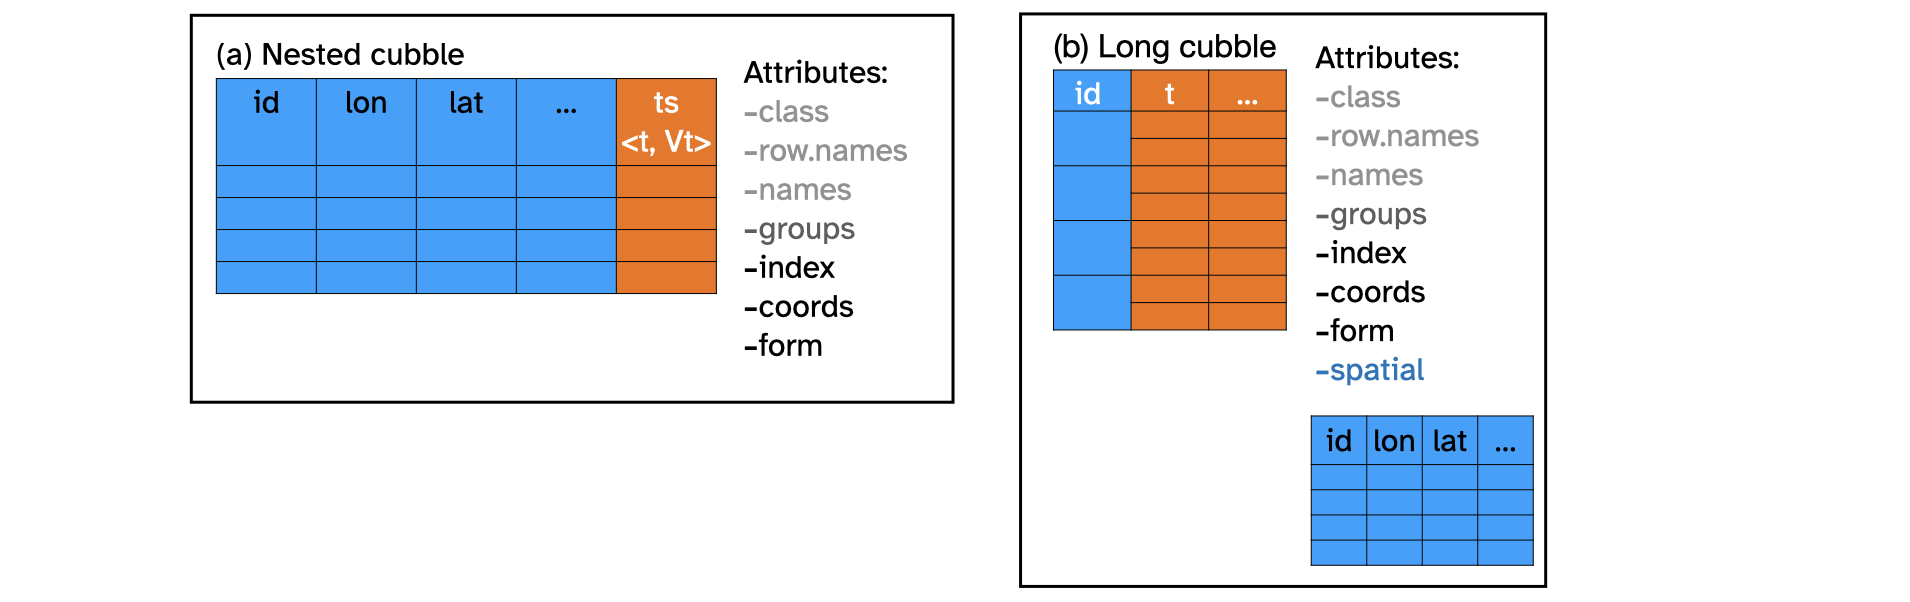
\includegraphics[width=1\linewidth]{../figures/diagram-keynotes/diagram-keynotes.002} 

}

\caption{An illustration of function \code{face\_temporal} and \code{face\_spatial}. In the first row, \code{face\_temporal} switches a \code{cubble} object from the nested form into the long form and the focus has switched from the spatial aspect (the side face) to the temporal aspect (the front face). In the second row, \code{face\_spatial} switches a \code{cubble} object back to the nested form from the long form and shifts focus back to the spatial aspect.}\label{fig:face}
\end{figure}
\end{CodeChunk}

Wrangling spatio-temporal data can be seen as an iterative process in the spatial and temporal dimensions. Switching the focus back to the site-variable face can be accomplished by the function \code{face_spatial()}, which is the inverse of \code{face_temporal()}. The second row of Figure \ref{fig:face} illustrates the function, which is used as follows:

\begin{CodeChunk}
\begin{CodeInput}
R> (cb_back <- cb_long |> face_spatial())
\end{CodeInput}
\begin{CodeOutput}
# cubble:   key: id [3], index: date, nested form
# extent:   [144.8321, -37.98, 145.0964, -37.6655]
# temporal: prcp [dbl], tmax [dbl], tmin [dbl]
  id           long   lat  elev name              wmo_id ts      
  <chr>       <dbl> <dbl> <dbl> <chr>              <dbl> <list>  
1 ASN00086038  145. -37.7  78.4 essendon airport   95866 <tibble>
2 ASN00086077  145. -38.0  12.1 moorabbin airport  94870 <tibble>
3 ASN00086282  145. -37.7 113.  melbourne airport  94866 <tibble>
\end{CodeOutput}
\begin{CodeInput}
R> #identical(cb_nested, cb_back)
\end{CodeInput}
\end{CodeChunk}

Sometimes, analysts may need to apply some variable transformation that involves both the spatial and temporal variables. An example of this is the transformation of temporal variables into the spatial dimension in glyph maps \citep{Wickham2012-yr}. (How to make glyph maps will be explained in Section \ref{st_transformation}, and are illustrated in the second example.) This type of operation can be seen as flattening, or \emph{unfolding}, the cube into a 2D data frame. Here the function \code{unfold()} moves the spatial variables \code{long} and \code{lat} into the long \code{cubble}:

\begin{CodeChunk}
\begin{CodeInput}
R> cb_long |> unfold(long, lat)
\end{CodeInput}
\begin{CodeOutput}
# cubble:  key: id [3], index: date, long form
# extent:  2020-01-01 -- 2020-01-10 [1D], no gaps
# spatial: long [dbl], lat [dbl], elev [dbl], name [chr], wmo_id
#   [dbl]
  id          date        prcp  tmax  tmin  long   lat
  <chr>       <date>     <dbl> <dbl> <dbl> <dbl> <dbl>
1 ASN00086038 2020-01-01     0  26.8  11    145. -37.7
2 ASN00086038 2020-01-02     0  26.3  12.2  145. -37.7
3 ASN00086038 2020-01-03     0  34.5  12.7  145. -37.7
4 ASN00086038 2020-01-04     0  29.3  18.8  145. -37.7
5 ASN00086038 2020-01-05    18  16.1  12.5  145. -37.7
# i 25 more rows
\end{CodeOutput}
\end{CodeChunk}

\hypertarget{compatibility-with-other-packages}{%
\subsection{Compatibility with other packages}\label{compatibility-with-other-packages}}

\subsubsection[]{\code{tsibble}}

The \code{tsibble} class is a subclass of \code{tibble} where the \code{index} and \code{key} components are used to store temporal and strata information, that makes working with temporal data cognitively efficient. A \code{cubble} object can use the \code{tsibble} class to store the temporal information, and effectively utilize the specialist time series operations in the \pkg{tsibble} package. A \code{tsibble} object can also be casted into a \code{cubble} object through supplying the coordinate information in the argument \texttt{coords}:

\begin{CodeChunk}
\begin{CodeInput}
R> cb <- make_cubble(
+   spatial = stations, temporal = meteo_ts, 
+   coords = c(long, lat))
\end{CodeInput}
\end{CodeChunk}

When a nested \code{cubble} is created, each element in the list-column \code{ts} is in the \code{tsibble} class (labelled \code{tbl_ts}) and operations available to the \code{tsibble} class are still valid on these elements. For example, the code below calculates two time series features (mean and variance) of maximum temperature, utilizing the \code{tsibble} syntax in the \code{cubble} object:

\begin{CodeChunk}
\begin{CodeInput}
R> cb %>% face_temporal() %>% tsibble::has_gaps()
\end{CodeInput}
\begin{CodeOutput}
# A tibble: 3 x 2
  id          .gaps
  <chr>       <lgl>
1 ASN00086038 FALSE
2 ASN00086077 FALSE
3 ASN00086282 FALSE
\end{CodeOutput}
\end{CodeChunk}

\subsubsection[]{\code{sf} (\code{s2})}

\emph{add an example on changing CRS?}

The \code{sf} class is also a subclass of \code{tibble} with a specialized feature geometry list-column (\code{sfc}) to store different geometry types (\code{POINT}, \code{LINESTRING}, \code{POLYGON}, \code{MULTIPOLYGON}, etc). The package \pkg{sf} provides functions that operate efficiently on this spatial information. A \code{cubble} object can store spatial information in the \code{sf} class. Methods for the \code{sfc} class can be applied in the nested form of the cubble object. An illustration is in Section \ref{covid}. The spatial information can also be stored as an \code{s2} vector in a \code{cubble} object.

\begin{CodeChunk}
\begin{CodeInput}
R> cb <- make_cubble(
+   spatial = stations_sf, temporal = meteo, 
+   key = id, index = date)
R> class(cb)
\end{CodeInput}
\begin{CodeOutput}
[1] "spatial_cubble_df" "cubble_df"         "sf"               
[4] "tbl_df"            "tbl"               "data.frame"       
\end{CodeOutput}
\begin{CodeInput}
R> #cb %>% sf::st_transform(crs = "EPSG:3857")
\end{CodeInput}
\end{CodeChunk}

\hypertarget{tidyverse}{%
\subsection{Comparison to other spatio-temporal classes}\label{tidyverse}}

Some readers may question why a new data structure is needed rather than directly creating a list-column on the combined data using \code{dplyr::nest_by()}. The reason is that the \code{cubble} object is specifically designed to utilize the spatio-temporal structure when arranging observations in a single object. Moreover, it enables easy pivoting between purely spatial, purely temporal, or unfolded into a combined form.

From the initial \pkg{spacetime} \citep{spacetime} package. New packages, such as \pkg{stars} \citep{stars} and \pkg{sftime} \citep{sftime}, have {[}\ldots{]}. This section compares and contrast the cubble data structure with other existing alternative, namely \pkg{stars} and \pkg{sftime}.

The \texttt{stars} package creates a \texttt{stars} object from an array and a dimension object. In many cases, i.e.~satellite images, this is convenient, however, there are also many spatio-temporal data are formatted in 2D data frames.

create a dimension object, populate the data into the array

\begin{itemize}
\tightlist
\item
  array in \proglang{R} allows for character,
\item
  specific datetime class
\end{itemize}

\emph{make the example simpler}

\begin{itemize}
\tightlist
\item
  \texttt{temporal\$var1\ \%\textgreater{}\%\ matrix(byrow\ =\ TRUE,\ nrow\ =\ 2,\ ncol\ =\ 5)}
\end{itemize}

This happens when different stations have different start date and require other software to reshape the data correctly.

The approach taken by the \pkg{sftime} package is to combine the spatial and temporal variables together into a joint table. {[}for sf objects with daily observation, memory efficiency{]}

Consider the climate data used in the \pkg{cubble} package, \code{climate_aus}. It contains daily precipitation, minimum and maximum temperature for 639 weather stations across Australia in 2020. The converted sftime object is times the size of the cubble object:

\begin{CodeChunk}
\begin{CodeInput}
R> #climate_aus %>% sftime::st_as_sftime() %>% object.size()
R> climate_aus %>% object.size()
\end{CodeInput}
\begin{CodeOutput}
8523040 bytes
\end{CodeOutput}
\end{CodeChunk}

\hypertarget{others}{%
\section{Other features and considerations}\label{others}}

\hypertarget{hierarchical-structure}{%
\subsection{Hierarchical structure}\label{hierarchical-structure}}

Spatial locations can have grouping structures either inherent to the data e.g., state within country or obtained during the analysis e.g., cluster id. In this case, it can be useful to summarize variables at various levels of the hierarchy. The function \code{switch_key()} can be used to change the grouping level of spatial locations. The diagram in Figure \ref{fig:illu-hier} shows how this function can be used to switch the grouping from station ids to cluster ids. The result can also be stretched into long form. By specifying \code{cluster_nested <- station_nested \%>\% switch_key(key = cluster)}, the \code{cubble} object redefines its \code{key} from the \code{id} column in \code{station_nested} to the \code{cluster} column in \code{cluster_nested}. All the spatial variables belonging to the \code{cluster} column are now nested into a \code{.val} column which allows for summarizing based on cluster.

\begin{CodeChunk}
\begin{figure}

{\centering 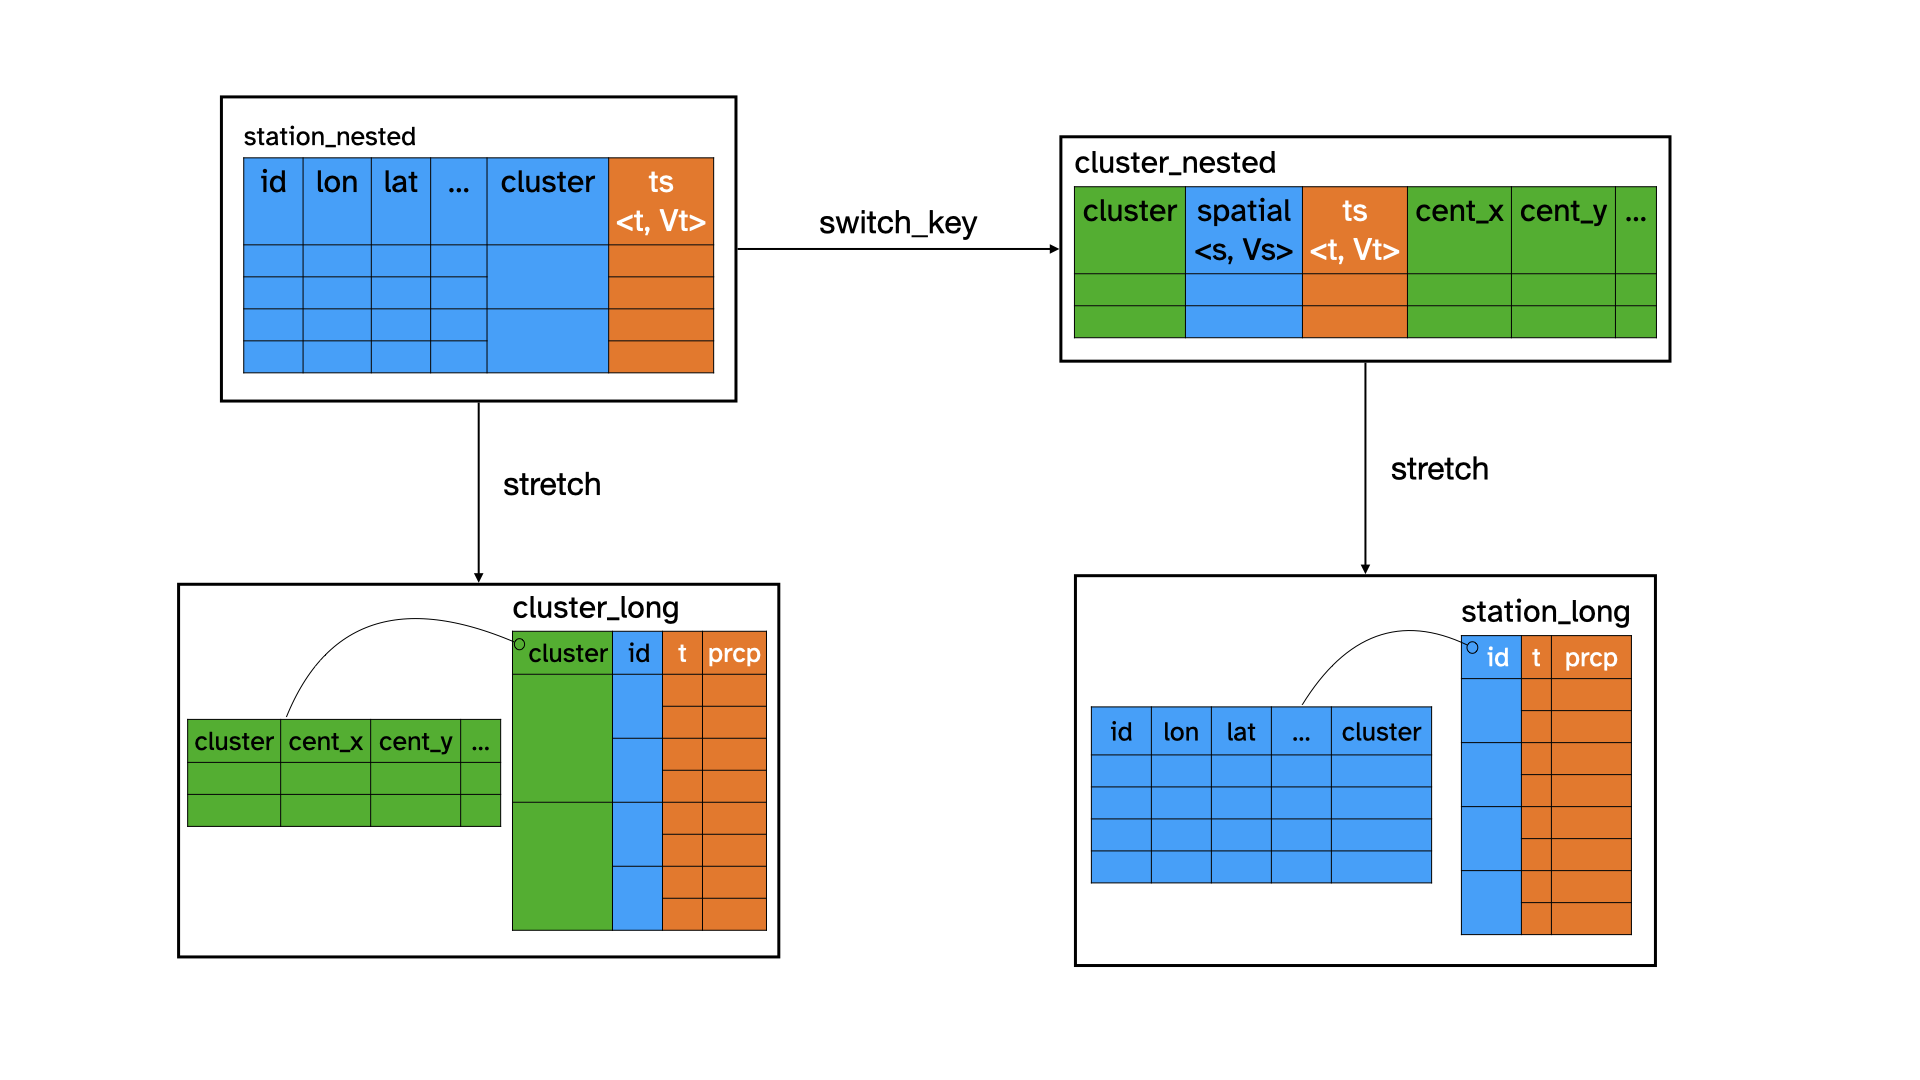
\includegraphics[width=1\linewidth,height=0.4\textheight]{../figures/diagram-keynotes/diagram-keynotes.003} 

}

\caption[Hierarchical spatial structure can be handled using \code{switch\_key()}, to create summaries based on any level]{Hierarchical spatial structure can be handled using \code{switch\_key()}, to create summaries based on any level. Here the switch is between the station id and a cluster id. Once the change is made the data can be stretched into the long form.}\label{fig:illu-hier}
\end{figure}
\end{CodeChunk}

\hypertarget{matching}{%
\subsection{Data fusion and matching}\label{matching}}

One task that may interest spatio-temporal analysts is combining data collected at nearby but not exactly the same sites, for example, weather station measured rainfall and river levels. This can be considered to be a matching problem \citep{stuart2010matching, mcintosh2018using} to pair similar time series from nearby locations, or even a data fusion exercise that merges data collected from different sources \citep{cocchi2019data}. The function \code{match_sites()} in the \pkg{cubble} package provides a simple algorithm for this task. The algorithm first matches spatially by computing the pairwise distance on latitude and longitude. Then it matches temporally by computing the number of matched peaks within a fixed length moving window. Figure \ref{fig:illu-matching} illustrates this temporal matching. In the two series, \emph{A} and \emph{a}, three peaks have been identified in each. An interval, of fixed length, is constructed for each peak in series \emph{A}, while the peaks in series \emph{a} are tested against whether they fall into any of the intervals. Here two out of three peaks match. Options for \code{match_sites()} are:

\begin{CodeChunk}
\begin{figure}

{\centering 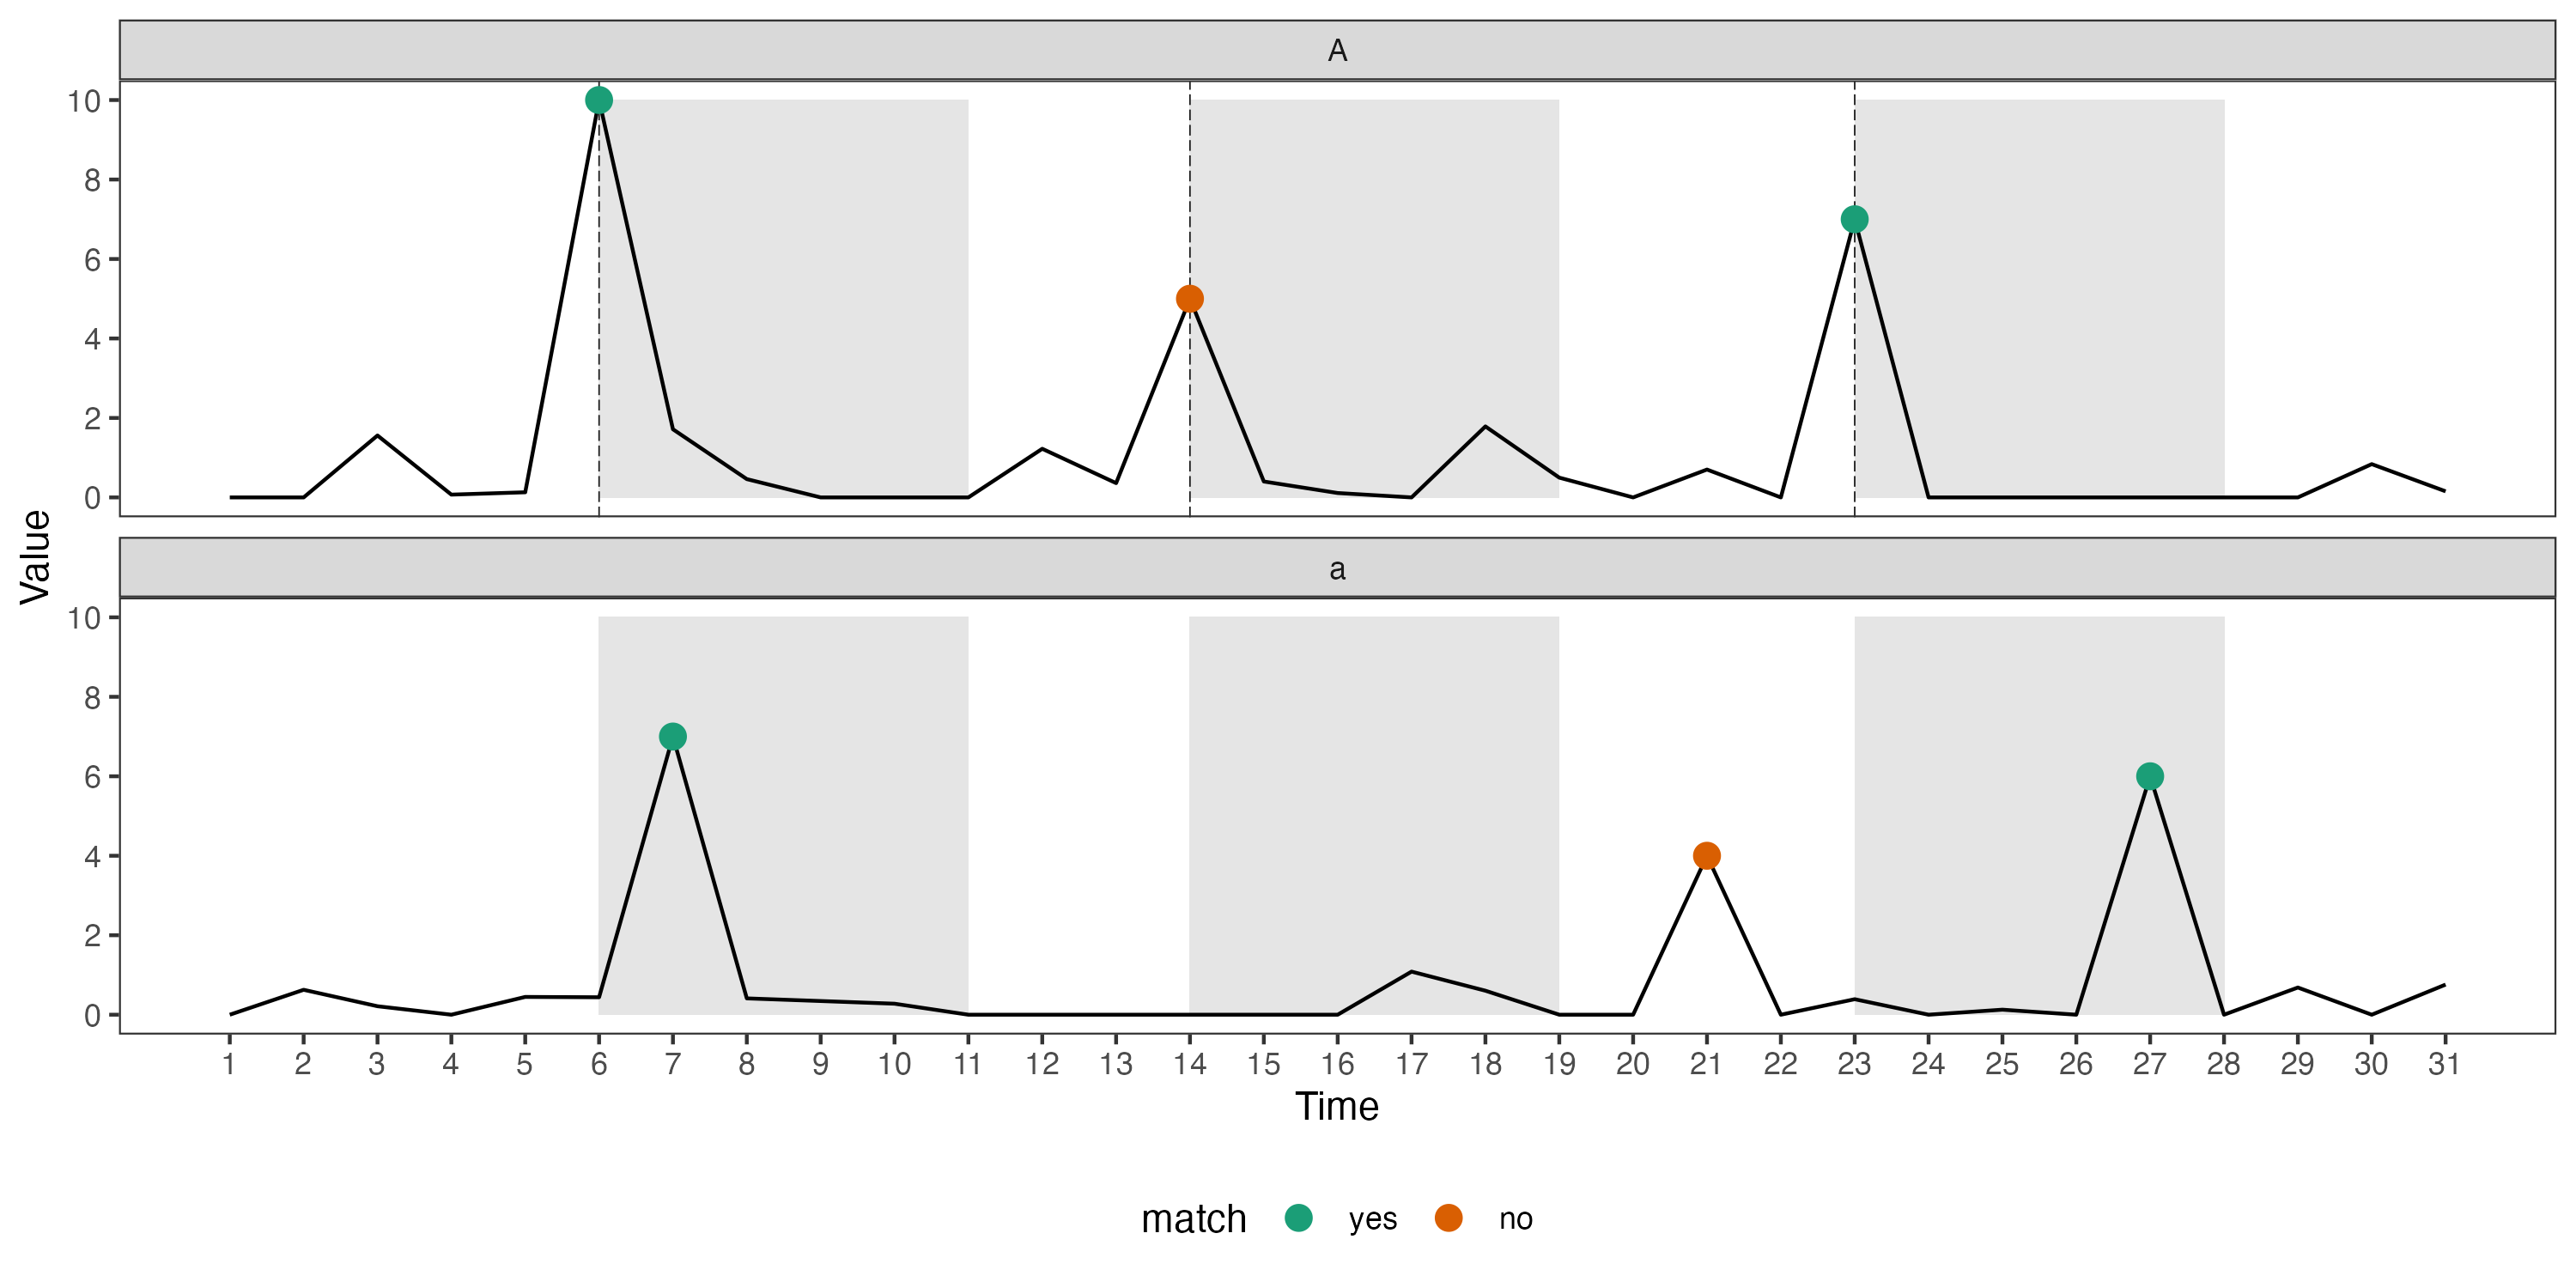
\includegraphics[width=1\linewidth]{../figures/illu-matching} 

}

\caption{An illustration of temporal matching in the \pkg{cubble} package. Three highest peaks are identified in each series and intervals are constructed on series \code{A}. Two peaks in series \code{a} fall into the intervals and hence the two series are considered to have two matches.}\label{fig:illu-matching}
\end{figure}
\end{CodeChunk}

\begin{itemize}
\tightlist
\item
  \code{spatial_n_keep}: the number of spatial match for each site to keep;
\item
  \code{spatial_dist_max}: the maximum distance allowed for a matched pair;
\item
  \code{temporal_n_highest}: the number of peaks used - 3 in the example above;
\item
  \code{temporal_window}: the length of the interval - 5 in the example above; and
\item
  \code{temporal_min_match}: the minimum number of matched peaks for a valid matched pair.
\end{itemize}

\hypertarget{interactive-graphics}{%
\subsection{Interactive graphics}\label{interactive-graphics}}

The workflow with the \code{cubble} class works well with an interactive graphics pipeline (e.g., \citet{buja1988elements}; \citet{buja1996interactive}; \citet{sutherland2000orca}; \citet{xie2014reactive}; \citet{cheng2016enabling}) that is available in \proglang{R} with the package \pkg{crosstalk} \citep{crosstalk}. Figure \ref{fig:illu-interactive} illustrates how linking can be achieved between a map and multiple time series in a \code{cubble} object. The map (produced from the nested form) and time series (produced from the long form) are both shared \code{crosstalk} objects. When a user makes a selection on the map, the site is highlighted (a). This activates a row in the nested \code{cubble}, which is then communicated to the long \code{cubble} -- all the observations with the same id (b) will be selected. The long \code{cubble} will then highlight the corresponding series in the time series plot (c).

Linking is also available starting from the time series plot, by selecting points. This will activate rows having the same id in the long \code{cubble}. The corresponding rows in the nested \code{cubble} are activated, and highlighted on the map. (An illustration can be found in the appendix.) Note that this type of linking, both from the map or the time series, is what \citet{CS07} would call categorical variable linking, where station id is the categorical variable.

\begin{CodeChunk}
\begin{figure}

{\centering 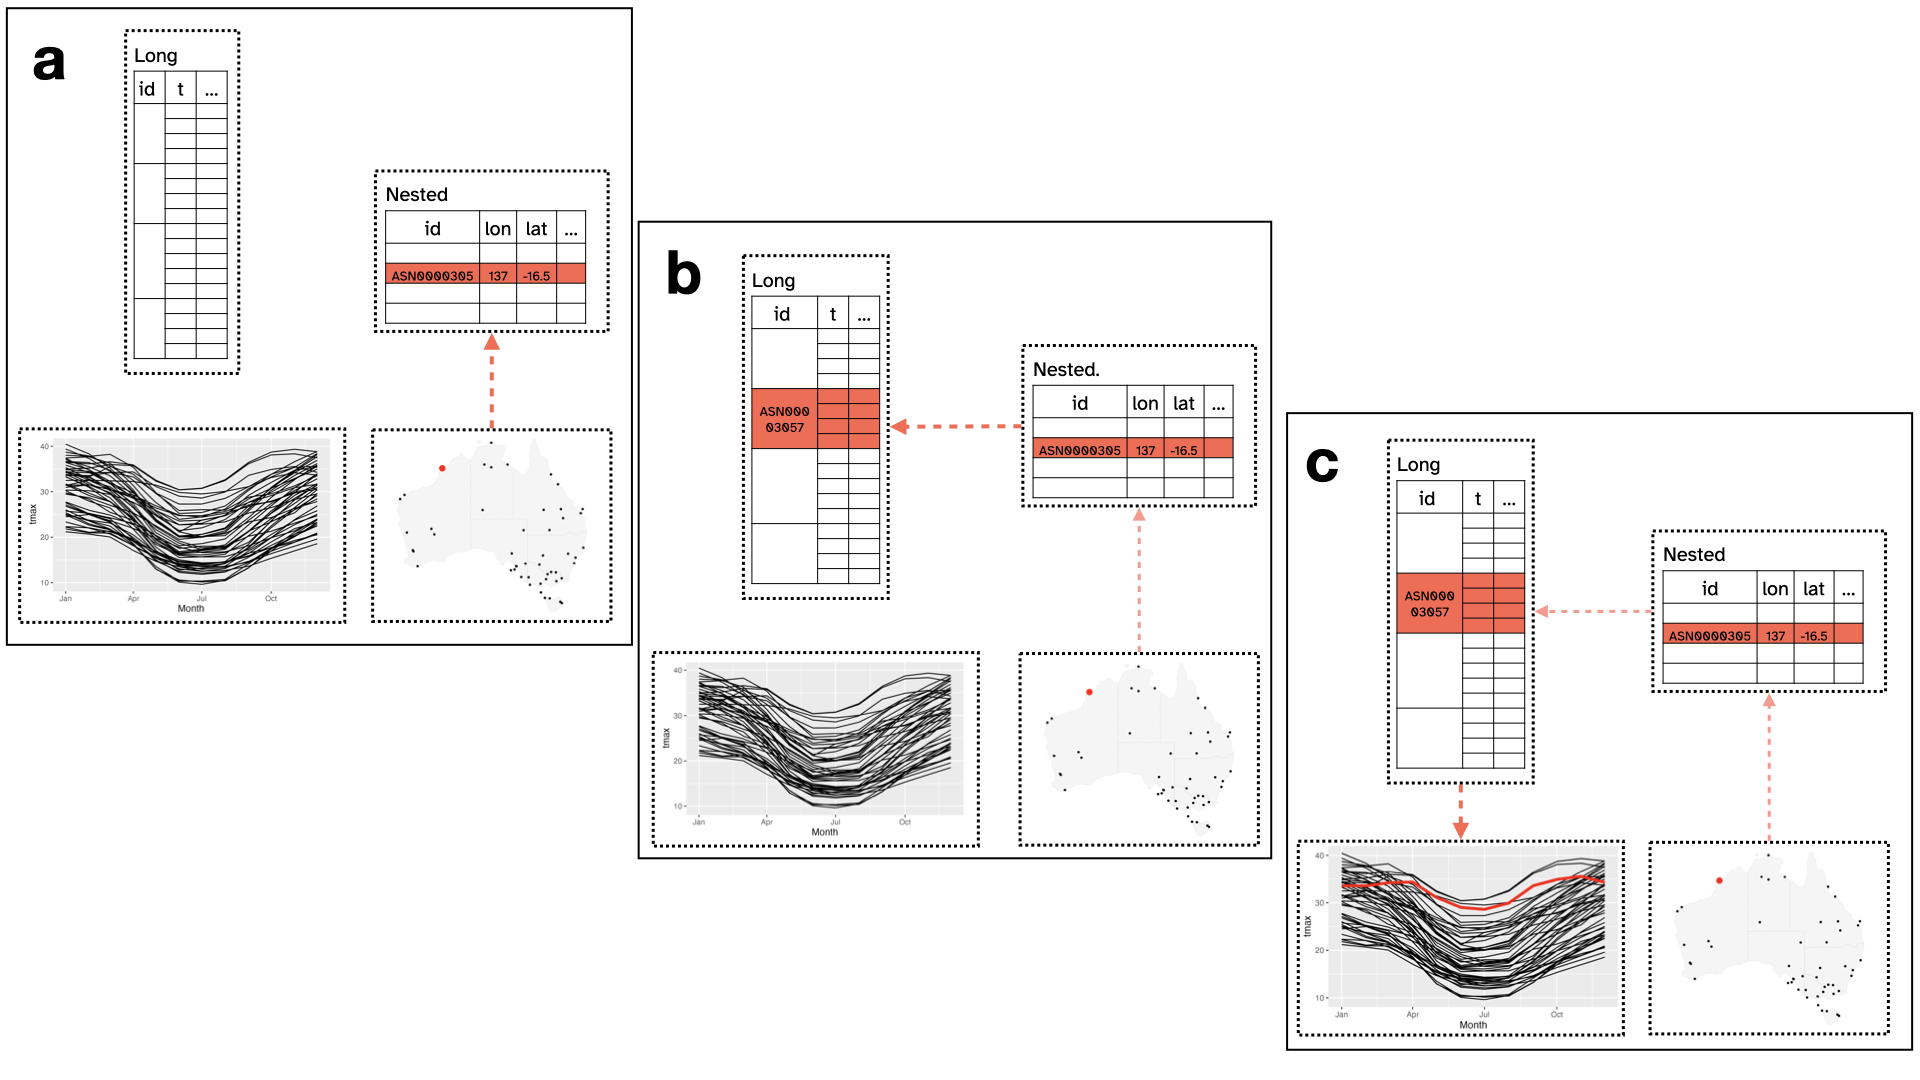
\includegraphics[width=1\linewidth,height=0.35\textheight]{../figures/diagram-keynotes/diagram-keynotes.004} 

}

\caption{Linking between multiple plots. The line plots and the map are constructed from shared \code{crosstalk} objects (long and nested \code{cubble}). When a station is selected on the map (a), the corresponding row in the nested \code{cubble} will be activated. This will link to all the rows with the same id in the long \code{cubble} (b) and update the line plot (c).}\label{fig:illu-interactive}
\end{figure}
\end{CodeChunk}

\hypertarget{st_transformation}{%
\subsection{Spatio-temporal transformations}\label{st_transformation}}

Spatio-temporal data lends itself to a range of transformations. Glyph maps \citep{Wickham2012-yr} transform the measured variable and time coordinates into microplots at the spatial locations. Calendar plots \citep{wang2020calendar} deconstruct time to produce plots of variables in a calendar format. Summarizing multiple variables is commonly done using projections, or linear combinations. Here we elaborate on the transformations made to produce a glyph map.

The package \pkg{GGally} \citep{ggally} has implemented glyph maps through the \code{glyphs()} function. The function constructs a \code{data.frame} with calculated position (\code{gx}, \code{gy}, \code{gid}) of each point on the time series using linear algebra (Equations 1 and 2 in \citet{Wickham2012-yr}). The data can then be piped into ggplot to create the glyph map as:

\begin{CodeChunk}
\begin{CodeInput}
R> library("ggplot2")
R> gly <- glyphs(data,
+               x_major = ..., x_minor = ...,
+               y_major = ..., y_minor = ..., ...)
R> 
R> ggplot(gly, aes(gx, gy, group = gid)) +
+   geom_path()
\end{CodeInput}
\end{CodeChunk}

A new implementation of the glyph map as a ggproto, \code{GeomGlyph}, has been made in the \pkg{cubble} package so that a glyph map can be created with \code{geom_glyph()}:

\begin{CodeChunk}
\begin{CodeInput}
R> ggplot(data = data) +
+   geom_glyph(aes(x_major = ..., x_minor = ...,
+                  y_major = ..., y_minor = ...))
\end{CodeInput}
\end{CodeChunk}

An example using a glyph map is shown in Section \ref{historicaltmax}.

Some useful controls over the glyph map are also available in the \code{geom_glyph()} implementation. Polar coordinate glyph maps are specified using \code{polar = TRUE}, and arguments \code{width} and \code{height} can be specified in either absolute or relative value. Global and local scale is specified with \code{global_rescale}, which defaults to \code{TRUE}. Reference boxes and lines can be added with separate \code{geom_glyph_box()} and \code{geom_glyph_line()} lines.

\hypertarget{examples}{%
\section{Applications}\label{examples}}

The five examples here are chosen to illustrate these aspects of the \pkg{cubble} package: creating a \code{cubble} object from two Coronavirus (COVID) data tables with the complication of differing location names, using spatial transformations to make a glyph map of seasonal temperature changes over years, aggregating information spatially to explore precipitation patterns, matching river level data and weather station records for analysis of water supply, reading NetCDF format data to reproduce a climate reanalysis plot, and the workflow to create complex interactive linked plots. (There is an additional example and figures in the Appendix, and more examples in the package vignettes.)

\hypertarget{covid}{%
\subsection{Victoria COVID spatio-temporal incidence and spread}\label{covid}}

Since the start of the pandemic, the Victoria State Government in Australia has provided daily COVID counts by local government area (LGA). This data can be used to visualize COVID incidence and spread spatially, when combined with map polygon data available from the Australian Bureau of Statistics. These different sources need to be combined for the analysis, by matching the LGA names. Here is how to do this with the \pkg{cubble} package, including how to handle mismatches arising from different names of the same LGAs in the two tables. The COVID data is store in a csv file and looks like:

\begin{CodeChunk}
\begin{CodeInput}
R> covid |> head(5)
\end{CodeInput}
\begin{CodeOutput}
# A tsibble: 5 x 5 [1D]
# Key:       lga [1]
# Groups:    lga, source [1]
  date       lga        source                            n roll_mean
  <date>     <chr>      <chr>                         <int>     <dbl>
1 2022-01-01 Alpine (S) Contact with a confirmed case     1        NA
2 2022-01-02 Alpine (S) Contact with a confirmed case     2        NA
3 2022-01-03 Alpine (S) Contact with a confirmed case     4        NA
4 2022-01-04 Alpine (S) Contact with a confirmed case     4        NA
5 2022-01-05 Alpine (S) Contact with a confirmed case     2        NA
\end{CodeOutput}
\end{CodeChunk}

and the spatial polygons are an ESRI shapefile as follows:

\begin{CodeChunk}
\begin{CodeInput}
R> lga |> head(5)
\end{CodeInput}
\begin{CodeOutput}
Simple feature collection with 5 features and 1 field
Geometry type: MULTIPOLYGON
Dimension:     XY
Bounding box:  xmin: 142.3535 ymin: -38.67876 xmax: 147.3909 ymax: -36.39269
Geodetic CRS:  WGS 84
               lga                       geometry
132     Alpine (S) MULTIPOLYGON (((146.7258 -3...
133    Ararat (RC) MULTIPOLYGON (((143.1807 -3...
134   Ballarat (C) MULTIPOLYGON (((143.6622 -3...
135    Banyule (C) MULTIPOLYGON (((145.1357 -3...
136 Bass Coast (S) MULTIPOLYGON (((145.5207 -3...
\end{CodeOutput}
\end{CodeChunk}

The function \code{make_cubble()} is used to create a \code{cubble} object from the two spatial and temporal tables, and requires specifying the arguments \code{key}, \code{index}, and \code{coords} (as described in Section \ref{create}). It will automatically try to match the sites in both tables using the location names and will show a warning message when there are mismatches, as shown below:

\begin{CodeChunk}
\begin{CodeInput}
R> cb <- make_cubble(spatial = lga, temporal = covid)
\end{CodeInput}
\begin{CodeOutput}
Warning: st_centroid assumes attributes are constant over geometries
\end{CodeOutput}
\begin{CodeOutput}
! Some sites in the spatial table don't have temporal information
\end{CodeOutput}
\begin{CodeOutput}
! Some sites in the temporal table don't have spatial information
\end{CodeOutput}
\begin{CodeOutput}
! Use `check_key()` to check on the unmatched key
The cubble is created only with sites having both spatial and temporal information
\end{CodeOutput}
\end{CodeChunk}

It can be seen that there are two-way mismatches -- LGAs in the COVID data that do not match with LGAs names in the spatial polygon data, and vice versa. The mismatches can be identified by using the function \code{check_key}:

\begin{CodeChunk}
\begin{CodeInput}
R> (check_res <- check_key(spatial = lga, temporal = covid))
\end{CodeInput}
\begin{CodeOutput}
$paired
# A tibble: 78 x 2
  spatial        temporal      
  <chr>          <chr>         
1 Alpine (S)     Alpine (S)    
2 Ararat (RC)    Ararat (RC)   
3 Ballarat (C)   Ballarat (C)  
4 Banyule (C)    Banyule (C)   
5 Bass Coast (S) Bass Coast (S)
# i 73 more rows

$potential_pairs
# A tibble: 2 x 2
  spatial             temporal    
  <chr>               <chr>       
1 Kingston (C) (Vic.) Kingston (C)
2 Latrobe (C) (Vic.)  Latrobe (C) 

$others
$others$spatial
[1] "No usual address (Vic.)"               
[2] "Migratory - Offshore - Shipping (Vic.)"

$others$temporal
[1] "Interstate" "Overseas"   "Unknown"   
\end{CodeOutput}
\end{CodeChunk}

With this information both tables can be fixed, to create the desired \code{cubble} object, as follows:

\begin{CodeChunk}
\begin{CodeInput}
R> lga2 <- lga |>
+   mutate(lga = ifelse(lga == "Kingston (C) (Vic.)", "Kingston (C)", lga),
+          lga = ifelse(lga == "Latrobe (C) (Vic.)", "Latrobe (C)", lga)) |>
+   filter(!lga %in% check_res$others$spatial)
R> 
R> covid2 <- covid |> filter(!lga %in% check_res$others$temporal)
R> 
R> (cb <- make_cubble(spatial = lga2, temporal = covid2))
\end{CodeInput}
\begin{CodeOutput}
# cubble:   key: lga [80], index: date, nested form, [sf]
# extent:   [140.961682, -39.1591895, 149.976291, -33.9804256]
# temporal: source [chr], n [int], roll_mean [dbl]
  lga             long   lat                       geometry ts        
  <chr>          <dbl> <dbl>             <MULTIPOLYGON [°]> <list>    
1 Alpine (S)      147. -36.9 (((146.7258 -36.45922, 146.80~ <gropd_ts>
2 Ararat (RC)     143. -37.5 (((143.1807 -37.73152, 143.17~ <gropd_ts>
3 Ballarat (C)    144. -37.5 (((143.6622 -37.57241, 143.66~ <gropd_ts>
4 Banyule (C)     145. -37.7 (((145.1357 -37.74091, 145.13~ <gropd_ts>
5 Bass Coast (S)  146. -38.5 (((145.5207 -38.30667, 145.54~ <gropd_ts>
# i 75 more rows
\end{CodeOutput}
\end{CodeChunk}

\hypertarget{historicaltmax}{%
\subsection{Australian historical maximum temperature}\label{historicaltmax}}

The GHCN provides daily climate measures from stations across the world. The data used here (\code{historical_tmax}) is a subset extracted using the package \pkg{rnoaa} \citep{rnoaa}, containing the records of maximum temperature for 237 Australian stations from \ensuremath{\infty{}} through \ensuremath{-\infty{}} and provides information also on the latitude, longitude and elevation of each of the stations. The goal of this example is to compare the monthly average maximum temperature between two periods, 1971-1975 and 2016-2020, for stations in Victoria and New South Wales (NSW), using a glyph map.

First, the stations need to be filtered to those in Victoria and NSW by using the station identifiers, stored within the 11 digits of the \code{id} variable entries. The country code is in the first 5 digits (Australia is represented by ``ASN00'') and the next 6 digits encode the station following the Australian Bureau of Meteorology (BOM) \citep{bom} coding protocols. The NSW stations correspond to entries in the range 46-75 and the Victorian stations to 76-90. Filtering Victoria and NSW stations is a \emph{spatial operation} and hence uses the nested \code{cubble}:

\begin{CodeChunk}
\begin{CodeInput}
R> tmax <- historical_tmax |>
+   filter(between(as.numeric(stringr::str_sub(id, 7, 8)), 46, 90))
\end{CodeInput}
\end{CodeChunk}

Next, the monthly maximum average temperature is calculated for both periods. This is a \emph{temporal operation} requiring a switch into the long \code{cubble} using the \code{face_temporal()} function. In addition, a new indicator for the two time periods of interest is created before the calculation of monthly averages:

\begin{CodeChunk}
\begin{CodeInput}
R> tmax <- tmax |>
+   face_temporal() |> 
+   group_by(
+     yearmonth = tsibble::make_yearmonth(
+       year = ifelse(lubridate::year(date) > 2015, 2016, 1971),
+       month = lubridate::month(date))
+     )|>
+   summarise(tmax = mean(tmax, na.rm = TRUE))
\end{CodeInput}
\end{CodeChunk}

A quick check on the number of observations for each location is made, revealing that there are several with less than 24 observations -- these stations lack temperature values for some months. In this example, those stations are removed by switching to a long \code{cubble} to operate on the spatial component over time, and then, move back into the nested \code{cubble} (to make the glyph map):

\begin{CodeChunk}
\begin{CodeInput}
R> tmax |> 
+   face_spatial() |> 
+   mutate(n = nrow(ts)) |>
+   arrange(n) |>
+   pull(n) |> 
+   head(10)
\end{CodeInput}
\begin{CodeOutput}
 [1] 12 12 12 13 19 19 20 24 24 24
\end{CodeOutput}
\begin{CodeInput}
R> tmax <- tmax |> 
+   face_spatial() |> 
+   filter(nrow(ts) == 24) |>
+   face_temporal()
\end{CodeInput}
\end{CodeChunk}

In order to create a glyph map displaying the monthly series (Figure \ref{fig:basic-manip}), the spatial variables need to be unfolded with the temporal variables. The reason being that the major (\code{long}, \code{lat}) and minor (\code{month}, \code{tmax}) coordinates need to be on the same table to create the glyph map. The \code{geom_glyph()} function does both the transformation and the plotting.

\begin{CodeChunk}
\begin{CodeInput}
R> nsw_vic <- ozmaps::abs_ste |>
+   filter(NAME %in% c("Victoria", "New South Wales"))
R> 
R> ggplot() +
+   geom_sf(data = nsw_vic,
+           fill = "transparent", color = "grey",
+           linetype = "dotted") +
+   geom_glyph(data = tmax,
+              aes(x_major = long, x_minor = month,
+                  y_major = lat, y_minor = tmax,
+                  group = interaction(id, group), color = group),
+              width = 1, height = 0.5) +
+   ...
\end{CodeInput}
\end{CodeChunk}

\begin{CodeChunk}
\begin{figure}

{\centering 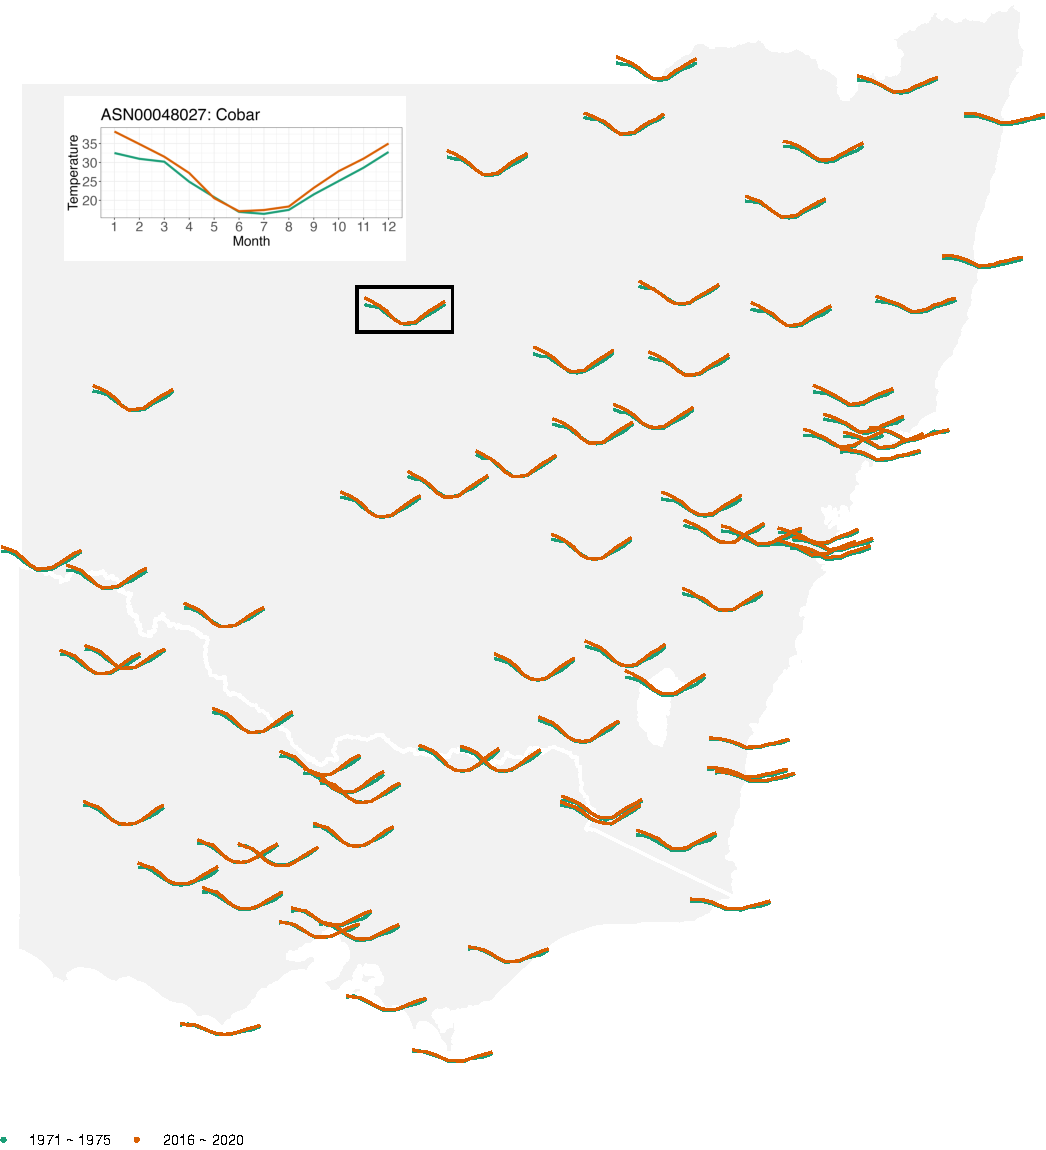
\includegraphics[width=1\linewidth]{/Users/hzha400/Documents/research/paper-cubble/figures/basic-manip-1} 

}

\caption[A glyph map of the monthly maximum average temperature for weather stations in  Victoria and New South Wales (NSW) for the periods (1971-1975, 2016-2020)]{A glyph map of the monthly maximum average temperature for weather stations in  Victoria and New South Wales (NSW) for the periods (1971-1975, 2016-2020). The corresponding average time series for the cobar station are display on the top left corner. From the glyph map we can observe that the monthly trend is similar for all locations (low in the winter, high in the summer), and small increased temperatures, particularly in late summer can be seen at most stations in NSW.}\label{fig:basic-manip}
\end{figure}
\end{CodeChunk}

Glyph maps work well to explore temporal patterns across spatial locations, particularly when the spatial locations are gridded. In this example, they are irregularly spaced, which can result in overlapping glyphs obscuring each other. To fix this, one could aggregate data from nearby stations. An example of this use is included in the Appendix.

\hypertarget{river-levels-and-rainfall-in-victoria}{%
\subsection{River levels and rainfall in Victoria}\label{river-levels-and-rainfall-in-victoria}}

River level and rainfall data for the same areas should have some similarity. Here we examine the river gauge data (\code{Water_course_level}) from the Bureau of Meteorology \citep{bom} in relation to weather station rainfall from NOAA's climate data (\code{climate}). The goal is to match water gauges with nearby weather stations, spatially and temporally, using the \code{match_sites()} function.

This function requires passing the major and minor data sets used for matching, in this case those are \code{river} and \code{climate}. The variables used for the temporal matching are \code{Water_course_level} from the \code{river} data set and \code{prcp} in the climate data set. The rest of the arguments, as explained in Section \ref{matching}, correspond to the maximum and minimum number of peaks in the time series to be matched. In this example those are set to be a maximum of 30 and a minimum of 15 (approximately 2 and 1 per month).

\begin{CodeChunk}
\begin{CodeInput}
R> res <- match_sites(
+   river, climate,
+   temporal_by = c("Water_course_level" = "prcp"),
+   temporal_independent = "prcp",  
+   temporal_n_highest = 30,
+   temporal_min_match = 15, 
+ )
\end{CodeInput}
\end{CodeChunk}

This function returns a \code{cubble} object, with additional columns: \code{dist} storing the distance between matched stations, \code{group} summarizing spatial matching, and \code{n_match} showing the temporal matching.

Figure \ref{fig:matching} shows four matched pairs on the map (a) and standardized data as time series (b). The expected concurrent increase in precipitation and water level can be seen clearly.

\hypertarget{era5-climate-reanalysis-data}{%
\subsection{ERA5: climate reanalysis data}\label{era5-climate-reanalysis-data}}

Figure \ref{fig:netcdf} reproduces the ERA5 data row of Figure 19 in \citet{hersbach2020era5}. Here we explain how this would be done using in the \pkg{cubble} package. The plots show that the southern polar vortex splits into two on 2002-09-26 and further splits into four on 2002-10-04. Further explanation of why this is interesting can be found in the figure source, and also in \citet{simmons2020global} and \citet{simmons2005ecmwf}.

The ERA5 data \citep{hersbach2020era5} provides hourly estimates across the Earth for atmospheric, land and oceanic climate variables. The data is available in the NetCDF format from the European Centre for Medium-Range Weather Forecasts (ECMWF). It can be directly downloaded from Copernicus Climate Data Store (CDS) \citep{cds} website or via the \pkg{ecmwfr} package \citep{ecwmfr}. For the reproduction, we focus on the \code{era5-pressure} data, hourly pressure levels from 1970 to present, with the \emph{specific humidity} and \emph{geopotential}. The downloaded NetCDF data (\texttt{raw}) is first converted to a \code{cubble} object:

\begin{CodeChunk}
\begin{CodeInput}
R> dt <- as_cubble(
+   raw, vars = c("q", "z"),
+   long_range = seq(-180, 180, 1), lat_range = seq(-88, 88, 1))
\end{CodeInput}
\end{CodeChunk}

Creating the plot requires making transformations on time, unfolding the data for computing the statistic of interest, which is plotted directly as a contour plot with ggplot. Code is provided to accomplish this in the supplementary material.

\begin{CodeChunk}
\begin{figure}

{\centering 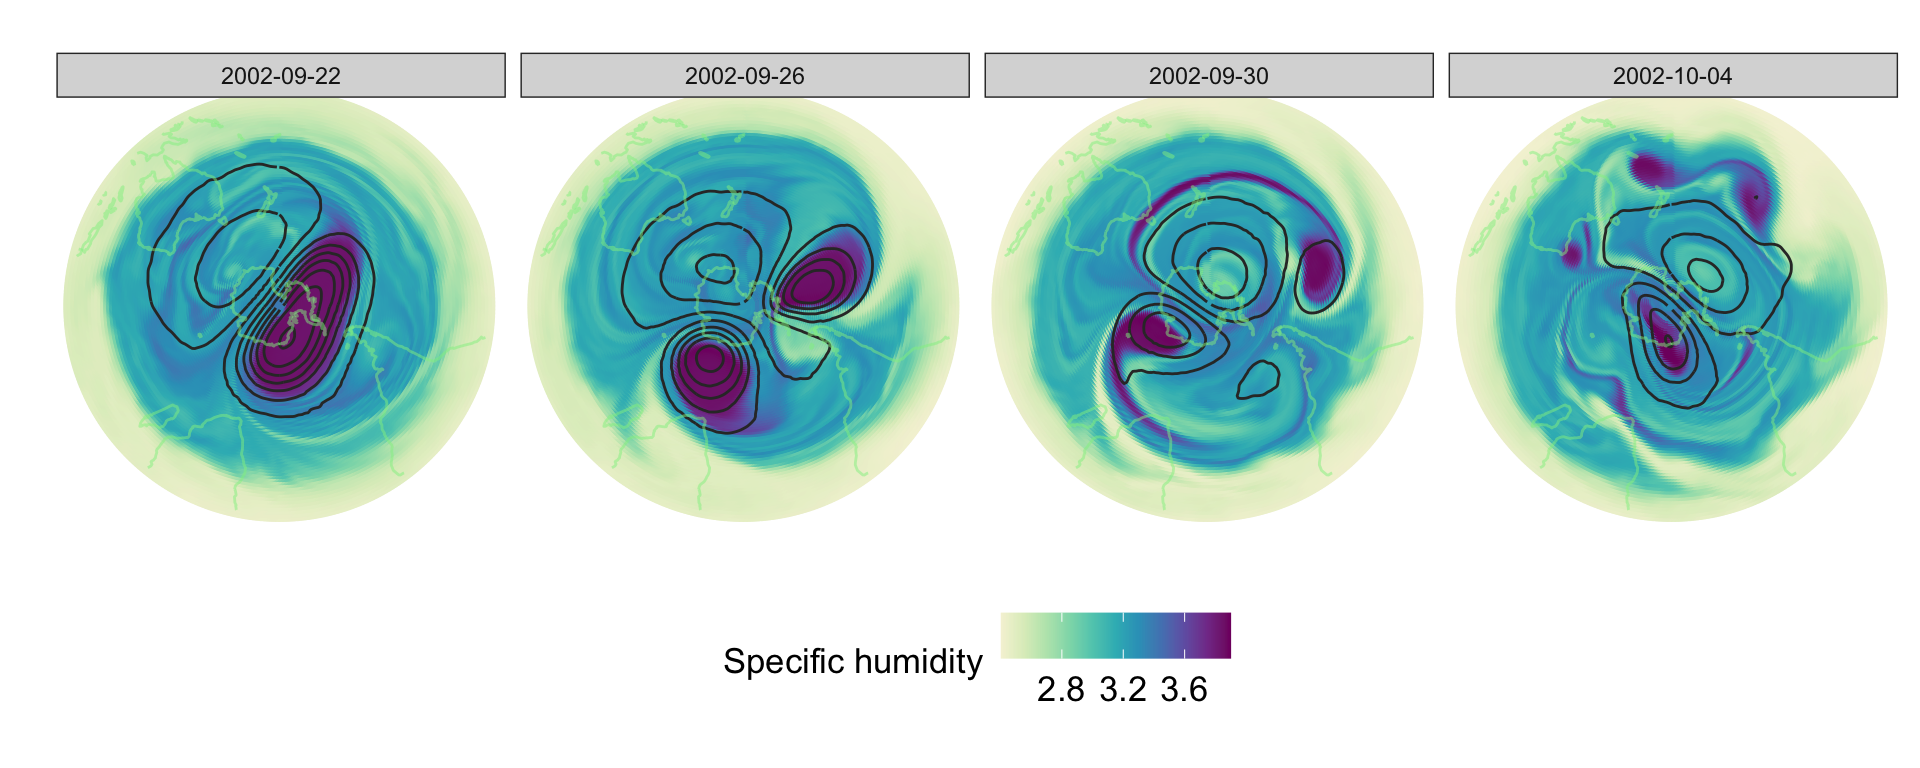
\includegraphics[width=1\linewidth]{/Users/hzha400/Documents/research/paper-cubble/figures/netcdf-1} 

}

\caption[A reproduction of the second row (ERA5 data) of Figure 19 in Hersbach et al (2020) to illustrate the break-up of sourthern polar vortex in late September and early October 2002]{A reproduction of the second row (ERA5 data) of Figure 19 in Hersbach et al (2020) to illustrate the break-up of sourthern polar vortex in late September and early October 2002. The polar vortex, signalled by the high specific humidity, splits into two on 2002-09-26 and further splits into four on 2002-10-04.}\label{fig:netcdf}
\end{figure}
\end{CodeChunk}

\hypertarget{interactive-graphics-1}{%
\subsection{Interactive graphics}\label{interactive-graphics-1}}

Interactive graphics can be useful because they make it possible to look at the data in multiple ways on-the-fly. This is especially important for spatio-temporal data, where we would like to interactively connect spatial and temporal displays. This example describes the process of using the \pkg{cubble} package with the \pkg{crosstalk} package to build an interactive display connecting a map of Australia, with ribbon plots of temperature range observed at the stations. The purpose is to explore the variation of monthly temperature range over the country. Figure \ref{fig:interactive-linking} shows three snapshots of the interactivity.

The key steps are to convert both the nested and long forms of the data into shared \code{crosstalk} objects, and to plot these side-by-side. The two are linked by the station identifier.

\begin{Shaded}
\begin{Highlighting}[]
\NormalTok{clean }\OtherTok{\textless{}{-}}\NormalTok{ climate\_full }\SpecialCharTok{|\textgreater{}}\NormalTok{ ...}

\NormalTok{nested }\OtherTok{\textless{}{-}}\NormalTok{ clean }\SpecialCharTok{|\textgreater{}}\NormalTok{ SharedData}\SpecialCharTok{$}\FunctionTok{new}\NormalTok{(}\SpecialCharTok{\textasciitilde{}}\NormalTok{id, }\AttributeTok{group =} \StringTok{"cubble"}\NormalTok{)}
\NormalTok{long }\OtherTok{\textless{}{-}} \FunctionTok{face\_temporal}\NormalTok{(clean) }\SpecialCharTok{|\textgreater{}}\NormalTok{ SharedData}\SpecialCharTok{$}\FunctionTok{new}\NormalTok{(}\SpecialCharTok{\textasciitilde{}}\NormalTok{id, }\AttributeTok{group =} \StringTok{"cubble"}\NormalTok{)}

\NormalTok{p1 }\OtherTok{\textless{}{-}}\NormalTok{ nested }\SpecialCharTok{|\textgreater{}}\NormalTok{ ...}
\NormalTok{p2 }\OtherTok{\textless{}{-}}\NormalTok{ long }\SpecialCharTok{|\textgreater{}}\NormalTok{ ...}

\NormalTok{crosstalk}\SpecialCharTok{::}\FunctionTok{bscols}\NormalTok{(plotly}\SpecialCharTok{::}\FunctionTok{ggplotly}\NormalTok{(p1), plotly}\SpecialCharTok{::}\FunctionTok{ggplotly}\NormalTok{(p2), ...)}
\end{Highlighting}
\end{Shaded}

Plot (a) shows the initial state of the interactive display: all locations are shown as dots on the map, coloured by temperature range, and the right plot shows the ribbons representing maximum to minimum for all stations. In plot (b) the ``Mount Elizabeth'' station, which shows a high variance colour on the initial map, is selected on the map and this produces the ribbon on the right. In plot (c) the lowest temperature in August is selected, which is ``Thredbo'' station on the left map. It was surprising to us that this was not a station in Tasmania, so for comparison a station in Tasmania is selected on the map to show in relation to Thredbo. We can see that Thredbo has a bigger winter dip in temperature, and although Tasmania is cold generally, it's temperatures are more constant

\begin{CodeChunk}
\begin{figure}

{\centering 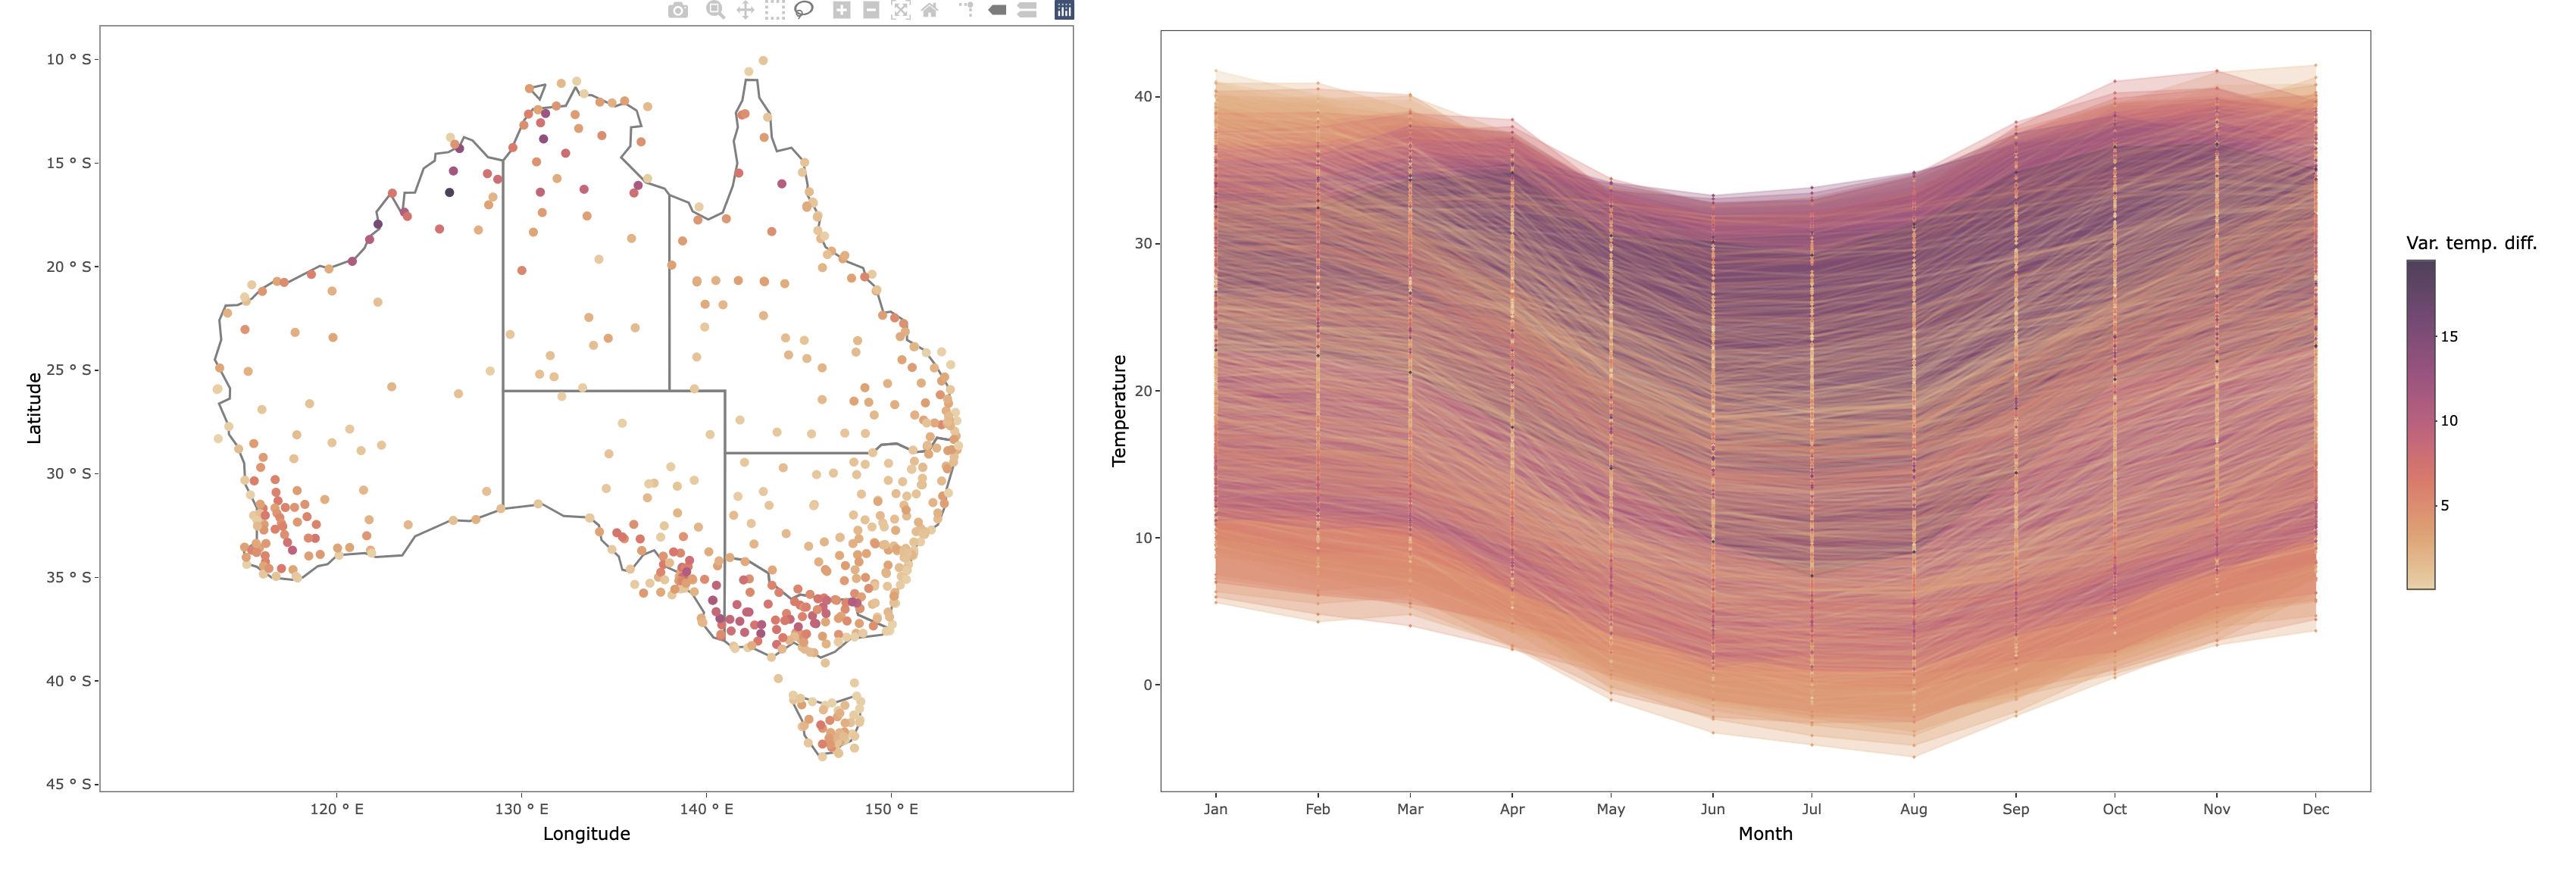
\includegraphics[width=1\linewidth,height=0.23\textheight]{../figures/linking} 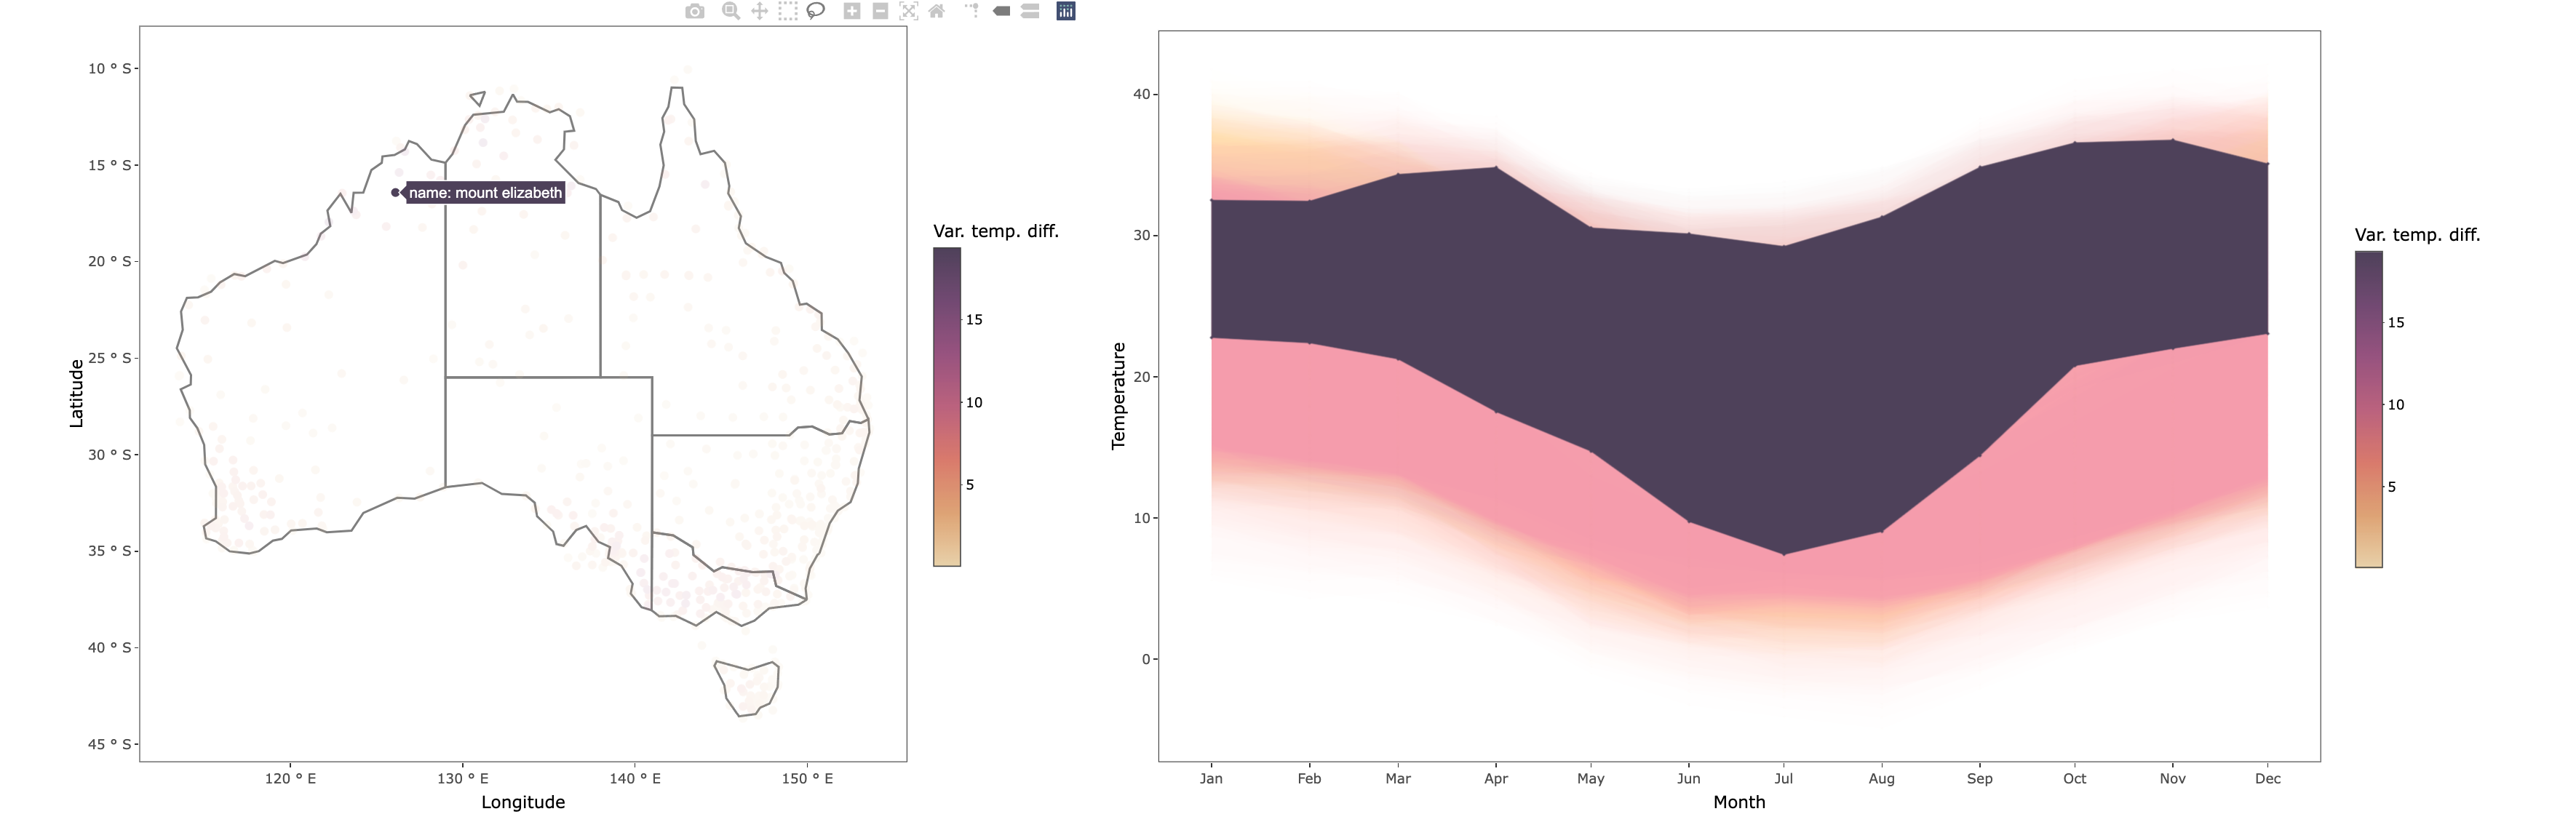
\includegraphics[width=1\linewidth,height=0.23\textheight]{../figures/linking-north} 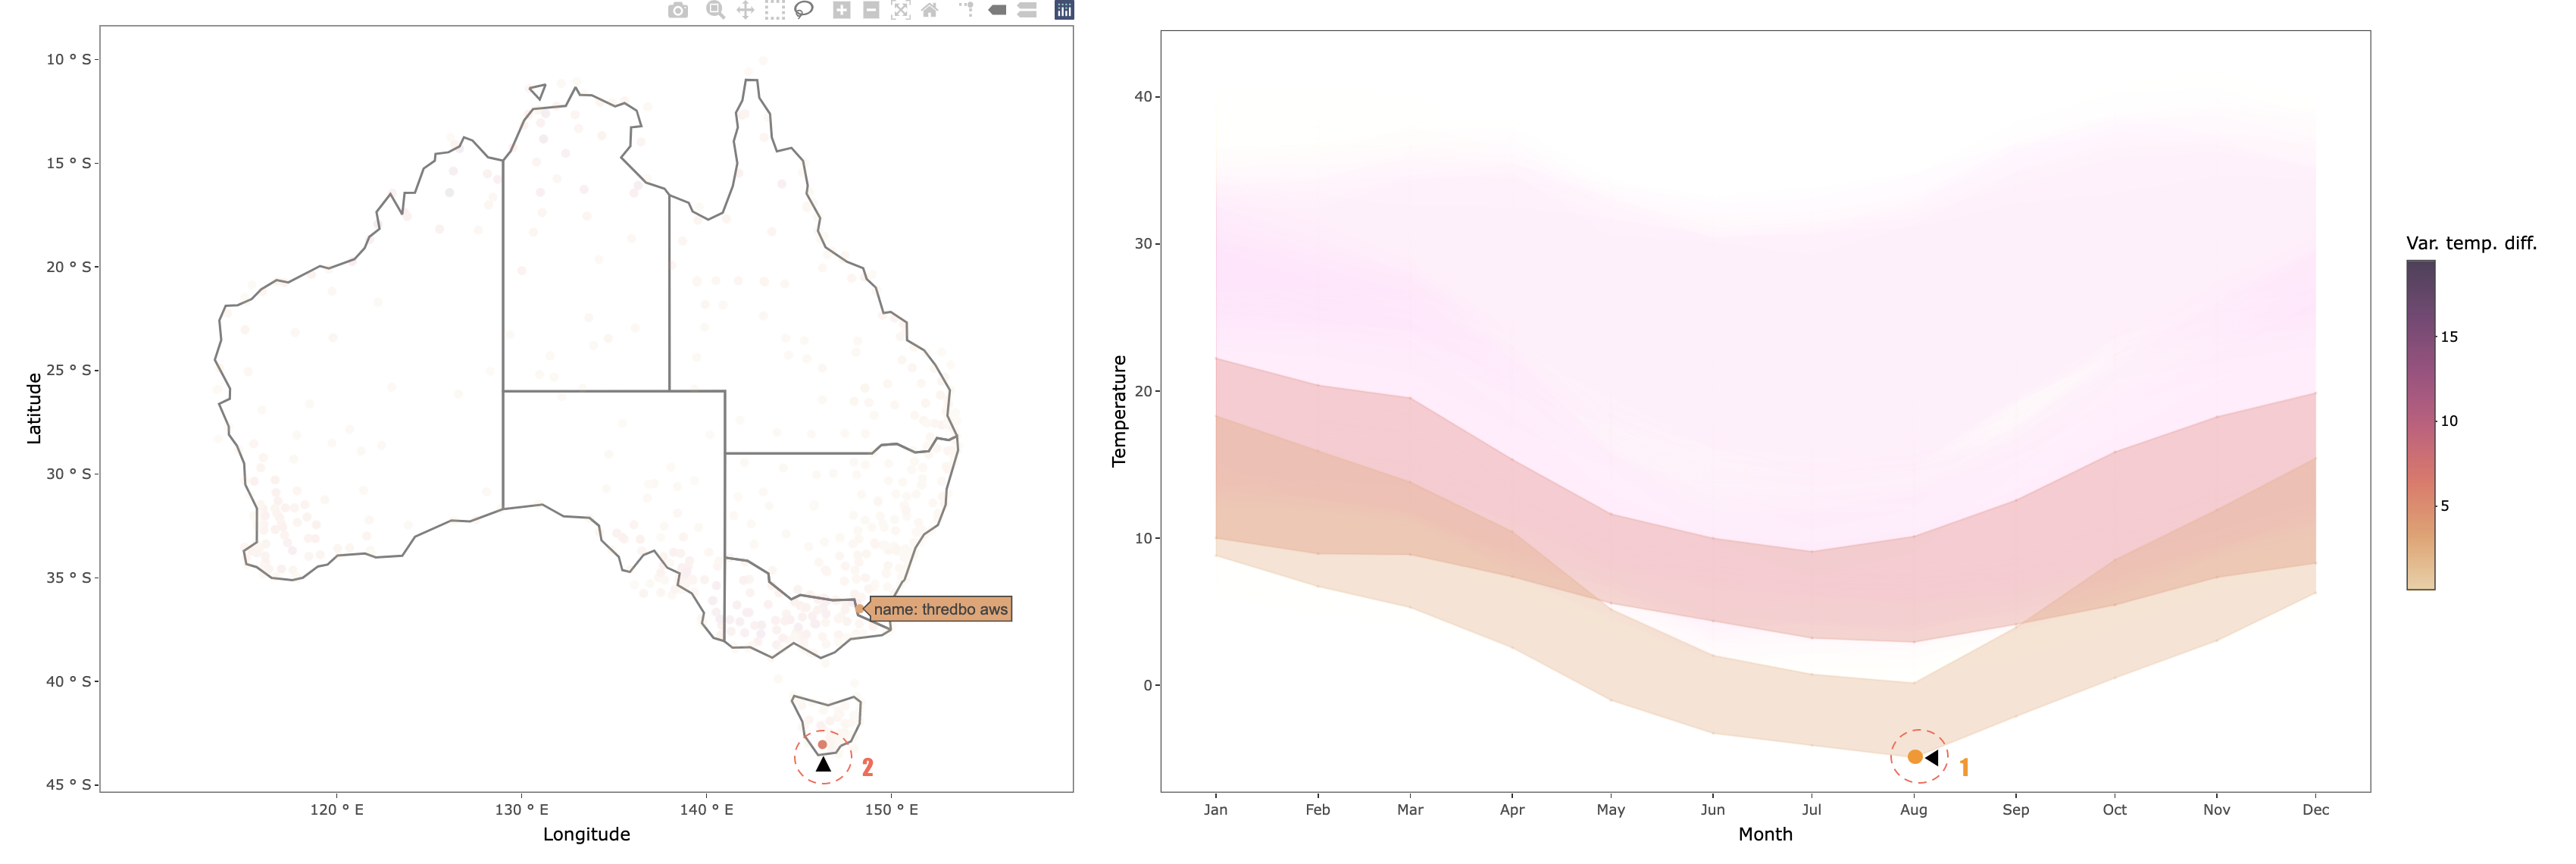
\includegraphics[width=1\linewidth,height=0.23\textheight]{../figures/linking-lower} 

}

\caption[Exploring temperature variation using linking of a map and seasonal display]{Exploring temperature variation using linking of a map and seasonal display. Each row is a screen dump of the process. The top row shows all locations and all temperature profiles. Selecting a particular location on the map (here Mount Elizabeth) produces the plot in the second row. The maximum and minimum temperatures are shown using a ribbon. The bottom row first selects the lowest temperature in August in the seasonal display, which highlights the corresponding station on the map (Thredbo). Another  station, located in the Tasmania Island, is then selected to compare its temperature variation with the Thredbo station.}\label{fig:interactive-linking}
\end{figure}
\end{CodeChunk}

\hypertarget{conclude}{%
\section{Conclusion}\label{conclude}}

This paper presents an \proglang{R} package \pkg{cubble} for organizing, manipulating and visualizing spatio-temporal data. The package introduces a new data class for spatio-temporal data, \code{cubble}, that connects the time invariant and varying variables and that allows the user to work with a nested and long form of the data. This work adds capabilities into the spatio-temporal practitioners toolbox to integrate it with a tidy data framework. The data structure and functions introduced in this package can be used and combined with existing spatial data analysis packages such as \pkg{sf}, data wrangling packages such as \pkg{dplyr}, and visualization packages such as \pkg{ggplot2}, \pkg{plotly} and \pkg{leaflet}.

Numerous examples are provided in the main text, appendix and package vignettes. These include creating and coercing data with mismatched names, handling hierarchical data, matching time series spatially and temporally, reproducing ERA5 plots from NetCDF data. Visualization of the \code{cubble} objects can be done with interactive graphic pipelines using \pkg{crosstalk}, \pkg{plotly} and \pkg{leaflet}.

There are several possible future directions for the work. The data structure only described fixed spatial sites, and it could be useful to provide tools to accommodate moving coordinates as might be encountered in animal movement data. That could be achieved with a list-column for the location coordinates, and an additional form that these locations can be pivoted into, like the long form for temporal variables. For multiple measured variables, the \pkg{cubble} package could be integrated with dimension reduction methods, and dynamic graphics for multiple dimensions such as a tour \citep{wickham_tourr_2011}.

\hypertarget{acknowledgement}{%
\section{Acknowledgement}\label{acknowledgement}}

This work is funded by a Commonwealth Scientific and Industrial Research Organisation (CSIRO) Data61 Scholarship and started while Nicolas Langrené was affiliated with CSIRO's Data61. The article is created using the package \pkg{knitr} \citep{knitr} and \pkg{rmarkdown} \citep{rmarkdown} in \proglang{R} with the \code{rticles::jss_article} template. The source code for reproducing this paper can be found at: \url{https://github.com/huizezhang-sherry/paper-cubble}.

\bibliography{../references.bib}



\end{document}
